%  LaTeX support: latex@mdpi.com
%  In case you need support, please attach all files that are necessary for compiling as well as the log file, and specify the details of your LaTeX setup (which operating system and LaTeX version / tools you are using).

%=================================================================
\documentclass[atmosphere,article,accept,moreauthors,pdftex]{Definitions/mdpi}

% If you would like to post an early version of this manuscript as a preprint, you may use preprint as the journal and change 'submit' to 'accept'. The document class line would be, e.g., \documentclass[preprints,article,accept,moreauthors,pdftex]{mdpi}. This is especially recommended for submission to arXiv, where line numbers should be removed before posting. For preprints.org, the editorial staff will make this change immediately prior to posting.

%--------------------
% Class Options:
%--------------------
%----------
% journal
%----------
% Choose between the following MDPI journals:
% acoustics, actuators, addictions, admsci, aerospace, agriculture, agriengineering, agronomy, ai, algorithms, animals, antibiotics, antibodies, antioxidants, applmech, applsci, arts, asc, asi, atmosphere, atoms, axioms, batteries, bdcc, behavsci , beverages, bioengineering, biology, biomedicines, biomimetics, biomolecules, biosensors, brainsci , buildings, cancers, carbon , catalysts, cells, ceramics, challenges, chemengineering, chemistry, chemosensors, children, civileng, cleantechnol, climate, clockssleep, cmd, coatings, colloids, computation, computers, condensedmatter, cosmetics, cryptography, crystals, dairy, data, dentistry, designs , diagnostics, diseases, diversity, drones, econometrics, economies, education, ejbc, ejihpe, electrochem, electronics, endocrines, energies, entropy, environments, epigenomes, est, fermentation, fibers, fire, fishes, fluids, foods, forecasting, forests, fractalfract, futureinternet, futurephys, galaxies, games, gastrointestdisord, gels, genealogy, genes, geohazards, geosciences, geriatrics, hazardousmatters, healthcare, hearts, heritage, highthroughput, horticulturae, humanities, hydrology, ijerph, ijfs, ijgi, ijms, ijtpp, informatics, information, infrastructures, inorganics, insects, instruments, inventions, iot, j, jcdd, jce, jcm, jcp, jcs, jdb, jfb, jfmk, jimaging, jintelligence, jlpea, jmmp, jmse, jne, jnt, jof, joitmc, jpm, jrfm, jsan, land, languages, laws, life, literature, logistics, lubricants, machines, magnetochemistry, make, marinedrugs, materials, mathematics, mca, medicina, medicines, medsci, membranes, metabolites, metals, microarrays, micromachines, microorganisms, minerals, modelling, molbank, molecules, mps, mti, nanomaterials, ncrna, ijns, neurosci, neuroglia, nitrogen, notspecified, nutrients, oceans, ohbm, optics, particles, pathogens, pharmaceuticals, pharmaceutics, pharmacy, philosophies, photonics, physics, plants, plasma, pollutants, polymers, polysaccharides, preprints , proceedings, processes, prosthesis, proteomes, psych, publications, quantumrep, quaternary, qubs, reactions, recycling, religions, remotesensing, reprodmed, reports, resources, risks, robotics, safety, sci, scipharm, sensors, separations, sexes, signals, sinusitis, smartcities, sna, societies, socsci, soilsystems, sports, standards, stats, surfaces, surgeries, sustainability, sustainableworld, symmetry, systems, technologies, telecom, test, tourismhosp, toxics, toxins, transplantology, tropicalmed, universe, urbansci, vaccines, vehicles, vetsci, vibration, viruses, vision, water, wem, wevj

%---------
% article
%---------
% The default type of manuscript is "article", but can be replaced by:
% abstract, addendum, article, benchmark, book, bookreview, briefreport, casereport, changes, comment, commentary, communication, conceptpaper, conferenceproceedings, correction, conferencereport, expressionofconcern, extendedabstract, meetingreport, creative, datadescriptor, discussion, editorial, essay, erratum, hypothesis, interestingimages, letter, meetingreport, newbookreceived, obituary, opinion, projectreport, reply, retraction, review, perspective, protocol, shortnote, supfile, technicalnote, viewpoint
% supfile = supplementary materials

%----------
% submit
%----------
% The class option "submit" will be changed to "accept" by the Editorial Office when the paper is accepted. This will only make changes to the frontpage (e.g., the logo of the journal will get visible), the headings, and the copyright information. Also, line numbering will be removed. Journal info and pagination for accepted papers will also be assigned by the Editorial Office.

%------------------
% moreauthors
%------------------
% If there is only one author the class option oneauthor should be used. Otherwise use the class option moreauthors.

%---------
% pdftex
%---------
% The option pdftex is for use with pdfLaTeX. If eps figures are used, remove the option pdftex and use LaTeX and dvi2pdf.

%=================================================================
\firstpage{1} 
\makeatletter 
\setcounter{page}{\@firstpage} 
\makeatother
\pubvolume{1}
\issuenum{1}
\articlenumber{1}
\pubyear{2021}
\copyrightyear{2021}
\externaleditor{Academic Editor: Nicholas Herold}
\datereceived{} 
\dateaccepted{} 
\datepublished{} 
\hreflink{doi:} % Please use \linebreak if need to do line break
%\updates{yes} % If there is an update available, un-comment this line

%% MDPI internal command: uncomment if new journal that already uses continuous page numbers
%\continuouspages{yes}

%------------------------------------------------------------------
% The following line should be uncommented if the LaTeX file is uploaded to arXiv.org
%\pdfoutput=1

%=================================================================
% Add packages and commands here. The following packages are loaded in our class file: fontenc, inputenc, calc, indentfirst, fancyhdr, graphicx,epstopdf, lastpage, ifthen, lineno, float, amsmath, setspace, enumitem, mathpazo, booktabs, titlesec, etoolbox, tabto, xcolor, soul, multirow, microtype, tikz, totcount, amsthm, hyphenat, natbib, hyperref, footmisc, url, geometry, newfloat, caption

\usepackage[export]{adjustbox}
\usepackage{url}

%=================================================================
%% Please use the following mathematics environments: Theorem, Lemma, Corollary, Proposition, Characterization, Property, Problem, Example, ExamplesandDefinitions, Hypothesis, Remark, Definition, Notation, Assumption
%% For proofs, please use the proof environment (the amsthm package is loaded by the MDPI class).

%=================================================================
% Full title of the paper (Capitalized)
\Title{A Multi-Fidelity Framework for Wildland Fire Behavior Simulations over Complex Terrain}
%Attention AE/ME. The following layout issues have not been checked by the English Editing Department and must be carefully verified by the AE/Layout Department: All callout issues, bold usage of callouts, and references to callouts in the text. Correct callout usage in figures. Figure and Table layout issues. Footnote formatting and Glossaries have not been checked. En dash usage for negative values, en dash usage to indicate relationships, en dash usage to indicate bonds (especially in chemistry). The English Editing Department is not responsible for correct italic usage for genes, proteins and technical terminology. This responsibility belongs to the authors. The following are also not checked: spacing between numbers and units of measurement, ratios, en dashes for ranges, date and time formats, punctuation in equation lines, and less than/more than spacing (< >). Finally, capitalization and layout of titles/headings must be properly checked as well as ensuring 'Eq.' and 'Fig.' are properly spelled out, as these are layout issues.

\TitleCitation{A Multi-Fidelity Framework for Wildland Fire Behavior Simulations over Complex Terrain}

% Author Orchid ID: enter ID or remove command
\newcommand{\orcidauthorA}{0000-0000-000-000X} % Add \orcidA{} behind the author's name
%\newcommand{\orcidauthorB}{0000-0000-000-000X} % Add \orcidB{} behind the author's name

% Authors, for the paper (add full first names)
\Author{Marcos Vanella$^{1,}$*, Kevin McGrattan $^{1,}$*, Randall McDermott $^1$, Glenn Forney $^1$, William Mell $^2$, Emanuele Gissi $^3$, and Paolo Fiorucci $^4$}

% Authors, for metadata in PDF
\AuthorNames{Marcos Vanella, Kevin McGrattan, Randall McDermott, Glenn Forney, William Mell, Emanuele Gissi, and Paolo Fiorucci}
\AuthorCitation{Vanella, M.; McGrattan, K.; McDermott, R.; Forney, G.; Mell, W.; Gissi, E.; Fiorucci, P.}

% Affiliations / Addresses (Add [1] after \address if there is only one affiliation.)
\address{%
$^{1}$ \quad National Institute of Standards and Technology, Gaithersburg, MD 20899, USA; kevin.mcgrattan@nist.gov (K.M.); randall.mcdermott@nist.gov (R.M.); glenn.forney@nist.gov (G.F.) \\
$^{2}$ \quad U.S. Forest Service, Seattle, Washington, WA 98103, USA; william.mell@usda.gov \\
$^{3}$ \quad Corpo nazionale dei Vigili del fuoco, Savona 17100, Italy; emanuele.gissi@vigilfuoco.it \\
$^{4}$ \quad CIMA Research Foundation, Savona 17100, Italy; paolo.fiorucci@cimafoundation.org}

% Contact information of the corresponding author
\corres{Correspondence: marcos.vanella@nist.gov, kevin.mcgrattan@nist.gov}


\abstract{A method for the large-eddy simulation (LES) of wildfire spread over complex terrain is presented. In this scheme, a cut-cell immersed boundary method (CC-IBM) is used to render the complex terrain, defined by a tessellation, on a rectilinear Cartesian grid. Discretization of scalar transport equations for chemical species is done via a finite volume scheme on cut-cells defined by the intersection of the terrain geometry and the Cartesian cells. Momentum transport and heat transfer close to the immersed terrain are handled using dynamic wall models and a direct forcing immersed boundary method. A new ``open'' convective inflow/outflow method for specifying atmospheric wind boundary conditions is presented. Additionally, three basic approaches have been explored to model fire spread: (1) Representing the vegetation as a collection of Lagrangian particles, (2) representing the vegetation as a semi-porous boundary, and (3) representing the fire spread using a level set method, in which the fire spreads as a function of terrain slope, vegetation type, and wind speed. Several test and validation cases are reported to demonstrate the capabilities of this novel wildfire simulation methodology.}

\keyword{complex terrain; fire spread; immersed boundary method; level sets}

\newcommand{\dV}{{\rm d}V}
\newcommand{\dS}{{\rm d}S}
\newcommand{\bx}{\mathbf{x}}
\newcommand{\bs}{\mathbf{s}}
\renewcommand{\C}{\mathrm{C}}
\renewcommand{\H}{\mathrm{H}}
\renewcommand{\O}{\mathrm{O}}

\begin{document}


\section{Introduction}

In the past few decades, wildland and wildland-urban interface (WUI) fires have received substantial attention due to their destructive nature and extensive cost to lives and property~\cite{thomas_2017,mcdermott_2019,richards_2020}. A~large body of literature can be found on the subject, as~seen in various review articles~\cite{Papadopoulos_2011,Bakhshaii_2019,mcdermott_2019}. Due to the complex nature of fire, limited computing resources, and~the needs of planners and first responders, most models of wildfires have historically relied on simplified field-tested rules and correlations. Among~these, the~rate of the spread model of Rothermel~\cite{Rothermel:1972} assumes quasi-steady-state surface fire conditions, and takes, as input, fuel properties, wind, terrain slope, and~moisture that can be measured in~situ. Fuel models have been cataloged~\cite{Anderson:1982}, and~their parameters defined so that model users can select and combine the most appropriate listed fuels. Rothermel's rate of spread formula is still widely used, and~has been implemented in several simulation tools~\cite{Finney:FARSITE,Bova:IJWF2015,FDS_Users_Guide,Coen:2,Coen:2015,LAUTENBERGER_2013,coen_2013,Mandel:2009,Mandel:2011,Mandel:2014,Kochanski:2016}, enabling a range of planning and operational forecasting~capabilities.

Wildland fire modeling typically focuses on tracking the fire front, which can have a complex shape that moves and deforms based on local conditions, like fuel loading, moisture content, wind, and~terrain. The~fire front requires a mathematical representation. The~Lagrangian approach is based on a polygonal mesh of control markers that represents the front~\cite{Finney:FARSITE,Bova:IJWF2015}. On~the other hand, an~Eulerian representation allows for a fixed two-dimensional mesh on which the fire front is defined implicitly by a scalar field. This scalar field is called the level set function, and numerical methods that compute the function are called level set methods (LSM)~\cite{Sethian:1999,Osher:2006}. Some wildfire solvers that use LSM to track the fire front are described in the References~\cite{coen_2013,Bova:IJWF2015,FDS_Users_Guide,LAUTENBERGER_2013}. A~practical comparison of the two techniques, as implemented in the Fire Dynamics Simulator (FDS)~\cite{Mell:IJWF2007} and FARSITE~\cite{Finney:FARSITE}, is provided in Ref.~\cite{Bova:IJWF2015}.

Because the spread rate of the fire front depends in part on the local wind conditions, a~well-resolved wind field over complex terrain should improve the accuracy of the overall model. The~de facto physics-based technique for practical simulation of wind is the Large Eddy Simulation (LES)~\cite{Linn:2007,coen_2013,Mell:IJWF2007}. For~fire simulation over complex terrain, a~range of techniques are being developed, in~particular, in~the coupling of the fire and the wind. For~fast simulation of outdoor fires, an~immersed boundary method has been interfaced with a level set scheme~\cite{Bova:IJWF2015} and the Rothermel fire spread model. The~wind speed input for Rothermel's model results from the local velocity over the terrain which is affected by fire buoyancy and flow evolution. These are, in turn, also influenced by wind atmospheric conditions, accounted for within simulations using a mean wind forcing concept. This is a first step at implementing a level set approach in an LES wind calculation with combustion. It is recognized that in the empirically based development of the Rothermel formula, the wind speed is not influenced by the local buoyancy-induced~flow.

A number of other approaches to modeling fire spread over complex terrain exist. A~recent review, with~an emphasis on operational applications, is given in~\cite{Arca_2019}. A~range of approximations to modeling both wind and fire have been employed. The~uniqueness of the approach presented here is that, within~a single computational tool, a~range of approximations to the wind and fire physics can be employed. This can support a direct comparison between models of varying physical fidelity. For~example, one can investigate the difference in predicted fire behavior between a simulation that models fire spread and heat release via the explicit accounting of the thermal degradation of vegetation and one that approximates fire spread via an empirically based~model. 

In the following section, the mathematical model for fire spread over complex terrain is described. The~description of the terrain discretization is provided in Section~\ref{sec:terraindisc}. The~various fire spread methods are described in Section~\ref{sec:firespread}, and~the atmospheric boundary conditions in Section~\ref{sec:wind}. Some flat terrain simulations are compared to experimental data, and~a complex terrain simulation is compared to an actual wildfire in Section~\ref{sec:numexp}. 


\section{Mathematical~Model} \label{sec:matmodel}
\unskip

\subsection{Governing~Equations} \label{sec:goveqns}

For fire modeling in the gas phase, FDS employs a low Mach approximation for thermally driven buoyant and stratified flows~\cite{Rehm:1}. Under~this assumption, the pressure field $p$ can be viewed as the summation of two components: a background hydrostatic pressure field $\bar{p}(z,t)$ used in the equation of state (ideal gas law), and a hydrodynamic pressure $\tilde{p}(x,y,z,t)$ driving fluid~motion.

Consider a mixture composed of $N$ chemical species $\alpha$, moving on a fixed point $\mathbf{x}$ in space with a mass weighted average velocity $\mathbf{u}(\mathbf{x},t)$. If~$\rho(\mathbf{x},t)$ is the mixture density, the~mass fraction for species $\alpha$ is $Y_\alpha = \rho_\alpha / \rho$, where $\rho_\alpha(\mathbf{x},t)$ is the species mass density and $\rho = \sum \rho_\alpha$. The~scalar transport and momentum equations take the form:
\begin{eqnarray}
   \frac{\partial \rho Y_\alpha}{ \partial t} + \nabla \cdot ( \rho Y_\alpha  \mathbf{u} ) &=& - \nabla \cdot \mathbf{J_{d}}_\alpha + \dot{m}_\alpha'''  +
    \dot{m}_{b,\alpha}'''\; , \; \alpha=1,\dots,N \label{eqn:spectran} \\
    \frac{\partial \mathbf{u}}{\partial t} - \mathbf{u} \times \boldsymbol{\omega} + \nabla H - \tilde{p} \, \nabla \left( 1/\rho\right) &=&
    \frac{1}{\rho} \left[ (\rho-\rho_0) \mathbf{g} + \mathbf{f}_{b} + \nabla \cdot \boldsymbol{\tau}^{dev} \right] \label{eqn:momtran},
\end{eqnarray}
where $\mathbf{J_{d}}_\alpha=- \rho D_\alpha \boldsymbol{\nabla} Y_\alpha$ is the diffusive flux for component $\alpha$. Fick's Law for binary diffusion with respect to a background species is assumed, and~$D_\alpha$ is the diffusivity of $\alpha$ with respect to the background species.  Mass fractions $Y_\alpha$, solution of equations~\eqref{eqn:spectran}, must obey realizability constraints $0<Y_\alpha<1$ and $\sum_\alpha Y_\alpha=1$. In~equations~\eqref{eqn:spectran} starting from a realizable solution, realizability implies $\sum_\alpha \mathbf{J_{d}}_\alpha = 0$. Therefore, to~enforce realizability, errors in diffusive transport are lumped into the most abundant species locally~\cite{McDermott:2015}. The~volumetric combustion source term for species $\alpha$ is $\dot{m}_\alpha'''(\mathbf{x},t)$;  the term $\dot{m}_{b,\alpha}'''$ is the contribution to species $\alpha$ from subgrid particle gasification. These correspond to the amount of mass per unit volume and time of species $\alpha$ being added or subtracted in a given point $\mathbf{x}$ due to chemical reaction or gasification of solid particles (or droplets), respectively.  Details of the combustion model are provided below in Section~\ref{sec:subgrid}.

In the momentum equation, the term $H=|\mathbf{u}|^2/2 + \tilde{p}/\rho$, $\tilde{p}$ is the perturbation pressure, and~$\rho_0(z)$ is the modeled height-dependent background density of the atmosphere.  \mbox{Additionally, $\boldsymbol{\omega}$ refers} to the vorticity field. The~gravity vector is $\mathbf{g}=(0,0,g_z)$, the~buoyancy force term is $ (\rho-\rho_0) \mathbf{g}$, $\mathbf{f}_{b}$ is the term contributed by modeled particle drag forces, and~$\boldsymbol{\tau}^{dev}$ is the deviatoric stress tensor accounting for molecular and subgrid turbulent stresses parameterized by an effective eddy viscosity model, discussed below in Section~\ref{sec:subgrid}.

Conservation of energy is achieved by forcing the flow field to obey the following thermodynamic divergence constraint:
\begin{eqnarray}
    ( \nabla \cdot \mathbf{u} )^{\rm th} &=&
    \left[ \frac{1}{\rho c_p T} - \frac{1}{\bar{p}} \right]
    \frac{\partial \bar{p}}{\partial t} + \frac{w \rho_0 g_z}{\rho c_p T} \nonumber \\
    &+& \frac{1}{\rho c_p T} \left[ \dot{q}''' + \dot{q}_b''' - \nabla \cdot \dot{\mathbf{q}}'' - \nabla \cdot \dot{\mathbf{q}}_{\rm r}'' - \mathbf{u} \cdot \nabla (\rho h_s) \right] \nonumber \\
    &+& \frac{1}{\rho} \sum_\alpha \left( \frac{\overline{W}}{W_\alpha} - \frac{h_{s,\alpha}}{c_p T} \right) \left[ \dot{m}_\alpha'''  + \dot{m}_{b,\alpha}''' - \nabla \cdot (\mathbf{J_{d}}_\alpha) - \mathbf{u} \cdot \nabla (\rho Y_\alpha) \right] \label{eq:divth},
\end{eqnarray}
where $h_{s,\alpha}$ is the sensible enthalpy of species $\alpha$, and $h_s$ is the sensible enthalpy of the mixture, $\dot{q}''', \dot{q}_b'''$ are heat release rates due to combustion and particle gasification, $T$ is the local gas temperature, and~$w$ is the local vertical velocity. The~mixture-specific heat at constant pressure and molecular weight are $c_p=\sum_{\alpha =1}^N{c_{p,\alpha} Y_\alpha}$ and $\overline{W}=\left(\sum_{\alpha =1}^N{Y_\alpha /W_\alpha} \right)^{-1}$, respectively. This thermodynamic divergence is derived from and acts as a proxy for the sensible enthalpy evolution equation~\cite{mcdermo_2014}. Equation~(\ref{eq:divth}) is derived by factoring the divergence from the sensible enthalpy equation and applying the ideal gas law.  Given a background pressure and a local mass density, the~local temperature is computed from the ideal gas law as $T = \bar{p} \overline{W} / (\rho R) $.

The term $\dot{\mathbf{q}}''$ in Equation~(\ref{eq:divth}) represents the conductive and diffusive heat fluxes discussed in Section~\ref{sec:subgrid}. The~net contribution from thermal radiation in the energy equation is defined by:
\begin{equation}
   -\nabla \cdot \dot{\mathbf{q}}_{\rm r}''(\bx) =
    \kappa(\bx) \, \left[ U(\bx) - 4 \pi \, I_{\rm b}(\bx) \right]  \quad ; \quad
    U(\bx) = \int_{4\pi} \, I(\bx,\bs') \, d\bs'  \label{simple_rte},
\end{equation}
where $\kappa(\bx)$ is the absorption coefficient, $I_b(\bx)$ is the source term, and~$I(\bx,\bs)$ is the solution of the radiation transport equation (RTE) for a non-scattering gray gas:
\begin{equation}
   \bs \cdot \nabla I(\bx,\bs) = \kappa(\bx) \; \left[ I_{\rm b}(\bx) - I(\bx,\bs) \right] \label{bandRTE1}.
\end{equation}

The source term, $I_{\rm b}$, requires special treatment because of the limited resolution of the underlying numerical grid in the vicinity of flames. In~large-scale fire simulations, \mbox{grid cells} are typically on the order of
tens of centimeters. Flame sheets cannot be resolved, meaning that the computed cell-average temperature can be significantly lower than temperatures one would expect to find in the reacting flame. Consequently, the~source term is approximated in grid cells where fuel and oxygen react. Elsewhere, the~subgrid temperature field is homogeneous, and the source term can be computed directly:
\begin{equation} \kappa I_{\rm b} = \left\{ \begin{array}{cll}
    \kappa \sigma T^4/\pi      & \hbox{Outside flame zone}, & \dot{q}'''=0  \\ [0.1in]
    C \kappa \sigma T^4/\pi  & \hbox{Inside flame zone}, & \dot{q}'''>0.
    \end{array} \right.  \label{radapprox1}
\end{equation}

The constant $C$ is computed at each time step so that the volume integral of \mbox{Equation~(\ref{simple_rte})} over the entire flaming region is approximately equal to the volume integral of $\chi_{\rm r} \,\dot{q}'''$ over that same region. Here, $\chi_{\rm r}$ is an empirical estimate of the {\em global} fraction of that energy emitted as thermal radiation. Typically, a~sooty fire radiates approximately one-third of the total combustion~energy.

The radiation equation is solved using a technique similar to a finite volume method for convective transport, thus the name given to it is the Finite Volume Method (FVM). Using approximately 100 discrete angles which are updated over multiple time-steps, the~finite volume solver requires about 20\% of the total CPU time of a calculation, a~modest cost given the complexity of radiation heat~transfer.

Section~\ref{particle_model} discusses how Lagrangian particles are used to represent vegetation like leaves, pine needles, and other subgrid objects. These particles absorb and emit thermal radiation, and~the underlying assumptions are described in that~section.

\subsection{Subgrid~Parameterizations} \label{sec:subgrid}

In the formal derivation of the LES equations (see, e.g,~\cite{Pope:2000,FDS_Tech_Guide}) the filtered nonlinear terms (advection terms, mean chemical source term, and~the unresolved boundary fluxes) require subgrid-scale parameterizations.  In~this section, LES filter notation, as well as Cartesian tensor index notation, are used to clarify the terms used in the governing~equations.

\subsubsection{Subgrid~Advection}

Unresolved turbulent eddies enhance the transport of mass, momentum, and~energy.  This added transport is accounted for with residual stresses and scalar fluxes.  The~subgrid-scale stress tensor is defined as
\begin{equation}
\tau_{ij}^{sgs} \equiv \bar{\rho}(\widetilde{u_i u_j} - \tilde{u}_i \tilde{u}_j),
\end{equation}
where an overline represents a volumetric filter and the tilde represents a Favre filter (\mbox{see, e.g.,~\cite{Poinsot:TNC}}).

In FDS, the deviatoric part of the subgrid stress tensor is modeled using the gradient diffusion hypothesis.  Thus, the~combined deviatoric stress may be written as follows:
\begin{equation}
\tau_{ij}^{dev} = \overline{\tau}_{ij} + \tau_{ij}^{sgs} - \frac{1}{3} \tau_{kk}^{sgs} = -2 (\mu + \mu_t) \left[ \tilde{S}_{ij} - \frac{1}{3} \tilde{S}_{kk} \right],
\end{equation}
where the symmetric rate-of-strain tensor is $S_{ij} \equiv \frac{1}{2}(\partial u_i/\partial x_j + \partial u_j/\partial x_i)$, and $\mu_t$ is an isotropic eddy viscosity.  Note that $\overline{\tau}_{ij}$ is already the deviatoric part of the molecular stress as the isotropic part is the pressure; $\mu$ is the molecular dynamic~viscosity.

The eddy viscosity $\mu_t$ is an important quantity in the simulation, as it affects all the turbulent transport and subgrid mixing time-scales, which, as~shown below, are crucial to the combustion model.  In~FDS, the~eddy viscosity is modeled as~\cite{Pope:2000,Deardorff:1980}
\begin{equation}
\mu_t = \bar{\rho} C_\nu \Delta \sqrt{k_{sgs}},
\end{equation}
with the constant taken as $C_\nu = 0.1$ (this value can be derived, assuming production equals dissipation and a model Kolmogorov spectrum~\cite{Pope:2000}; the model is also tested against decaying isotropic turbulence~\cite{CBC}).  In~practice, the~filter scale $\Delta$ is taken as the cube root of the cell volume.  Deardorff~\cite{Deardorff:1980} solved a transport equation for the subgrid kinetic energy per unit mass, $k_{sgs}$, in~order to account for subgrid buoyancy. In~FDS, the~density field is sufficiently resolved to account for buoyant plume accelerations, and~therefore it is found that an algebraic closure for $k_{sgs}$ is sufficient.  Following the work of Bardina~\cite{Bardina:1980}, a~scale-similarity idea is used; the subgrid kinetic energy per unit mass is modeled \mbox{as follows}:
\begin{equation}
k_{sgs} = \frac{1}{2}(\tilde{u}_i - \hat{\tilde{u}}_i)(\tilde{u}_i - \hat{\tilde{u}}_i),
\end{equation}
where the hat represents a test filter at a scale $2\Delta$.  For~the first Cartesian cell off the wall, where a test filter is not well-defined, the~eddy viscosity is taken from the WALE model~\cite{Nicoud:1999}.

Subgrid advection of mass and heat are also modeled using gradient diffusion.  The~turbulent diffusivities use constant turbulent Schmidt and Prandtl numbers, both set to 0.5; this simplification is justified based on high-resolution simulations of fire plumes (\mbox{see, e.g.,~\cite{Maragkos:2020}}). For~mass diffusion of species $\alpha$ in direction $i$, the flux is
\begin{equation}
J_{\alpha,i} = \bar{J}_{\alpha,i} + J_{\alpha,i}^{sgs} = -\bar{\rho}(D_\alpha + \frac{\mu_t}{\mathrm{Sc}_t}) \frac{\partial \tilde{Y}_\alpha}{\partial x_i}.
\end{equation}
Effective thermal conductivity and mass diffusivity are used in the heat flux, which may be written as
\begin{equation}
{\dot{q}''}_i = -(\bar{k} + \frac{\mu_t \bar{c}_p}{\mathrm{Pr}_t}) \frac{\partial \widetilde{T}}{\partial x_i} - \sum_\alpha \tilde{h}_{{\rm s},\alpha} ( \bar{\rho} D_\alpha + \frac{\mu_t}{\mathrm{Sc}_t} ) \frac{\partial \tilde{Y}_\alpha }{\partial x_i}.
\end{equation}

\subsubsection{Filtered Chemical Source~Term}

FDS treats combustion chemistry using a simplified approach.  Only fuel, air, and~products, referred to as ``lumped species'', are tracked.  Lumped species are groups of species that transport and react together and are always found in the same proportion.  For~example, air is a lumped species made up of 23 \% O$_2$ and 77 \% N$_2$ by mass.  For~vegetation, a~surrogate hydrocarbon, fuel, is usually assumed.  For~example, cellulose may be assumed to decompose to a volatile fuel gas with the formula $\C_{6} \H_{10} \O_{5}$.  The~products are defined stoichiometrically, often including prescribed yields of soot (for smoke) and carbon monoxide that may be obtained from empirical relationships for the specific fuel or from other sources (e.g., \cite{SFPE:Mulholland}).  Then, usually, a~single reaction is tracked (more complicated reaction schemes are possible in the code, but~for this work, a single reaction is sufficient):
\begin{equation}
\mathrm{Fuel} + s \, \mathrm{Air} \rightarrow (1+s) \,\mathrm{Products},
\end{equation}
where $s$ is the mass stoichiometric~coefficient.  

In LES of turbulent combustion, the filtered chemical source term, $\overline{\dot{m}_\alpha'''}$, is unclosed because the reaction kinetics are nonlinear functions of species concentration and temperature.  However, since the heat-releasing reactions in a fire are extremely fast compared to the time scales for turbulent mixing, it is common practice in fire dynamics simulations to utilize the eddy dissipation model of Magnussen and Hjertager~\cite{Magnussen:1} (see also~\cite{Poinsot:TNC}).  The~mass production term for the fuel species is written as
\begin{equation}
\overline{\dot{m}_{F}'''} = -\bar{\rho} \,\frac{\min(\tilde{Y}_F,\tilde{Y}_A/s)}{\tau_{mix}}.
\end{equation}

This formula states that the fuel is consumed at a rate proportional to the local limiting reactant concentration, and inversely proportional to the local mixing time-scale.  This is the so-called ``mixed is burnt'' approximation.  The~mixing time-scale is given by $\tau_{mix} = \min(\tau_d, \tau_u,\tau_g)$ \cite{McDermott:2011}, where the time-scales for diffusion, turbulent advection, and~gravitational acceleration are, respectively,
\begin{align}
\tau_d &= \Delta^2/D_F \\
\tau_u &= C_u \Delta / \sqrt{(2/3)k_{sgs}} \\
\tau_g &= \sqrt{2\Delta/g}.
\end{align}

Here, $D_F$ is the binary diffusivity of the fuel species in air, $k_{sgs}$ is the modeled subgrid kinetic energy per unit mass discussed above, and~$g$ is the gravitational acceleration. The~constant $C_u=0.4$ is determined by matching flame height correlations across a wide range of fire Froude numbers~\cite{FDS_Tech_Guide}.

The remaining mass production rates are found from stoichiometry.  The~local heat release rate, $\dot{q}'''$, an~important term in Equation~(\ref{eq:divth}), is then determined from
\begin{equation}
\label{eq:qdotppp}
\dot{q}''' = - \sum_\alpha \overline{\dot{m}_\alpha'''} \Delta h_{f,\alpha},
\end{equation}
where $\Delta h_{f,\alpha}$ are the heats of formation for each lumped species $\alpha$.

\paragraph{Flame Extinction} One of the advantages of a physics-based tool like FDS is the possibility of building into the model the effects of defensive actions on the fire spread rate.  FDS uses simple empirical rules to predict local extinction within a gas phase grid cell based on resolved species concentrations and the mean cell temperature. The~rules are based on the concept of a critical flame temperature. The~basic theory behind the critical flame temperature is described in~\cite{SFPE:Beyler}.  In~brief, if~the local heat release given by Equation~(\ref{eq:qdotppp}) is not sufficient to raise the cell temperature above the CFT, then $\overline{\dot{m}_{F}'''}$ is set to zero for that cell for that time-step.  Note that the flame extinction model does not directly affect surface cooling or smothering of the vegetative fuel, which may happen with certain fire suppression activities. However, such tactics can be accounted for through modifications to the solid fuel thermal degradation model discussed~below.

\subsubsection{Unresolved Boundary~Fluxes}
\label{sec:boundflx}
In this section, the~wall functions used to close the mass, momentum, and~energy fluxes on solid boundaries are discussed.  Mass transfer of moisture and fuel from the surface is discussed in more detail below in Section~\ref{sec:firespread}, where the various flames spread models are compared (which is really the main focus of this paper).

The scaled streamwise velocity is denoted $u^+ = u/u_\tau$, where the friction velocity is $u_\tau \equiv \sqrt{\tau_w/\rho}$ and $\tau_w$ is the wall stress needed to close the momentum equation, \mbox{Equation~(\ref{eqn:momtran})}.  For~rough walls, FDS employs the log law presented in~\cite{Pope:2000},
\begin{equation}
\label{eqn_roughwallloglaw}
u^+ = \frac{1}{\kappa} \ln \left(\frac{y}{s}\right) + \tilde{B}(s^+),
\end{equation}
where $\kappa = 0.41$ is the von K\'arm\'an constant, $s^+ = s/\delta_\nu$ is the roughness length in viscous units, $s$ is the dimensional ``sand grain'' roughness, and~$\delta_\nu = \mu/(\rho u_\tau)$ is the viscous length scale. The~distance to the wall, $y$, is taken as $\delta y/2$ for the first off-wall grid cell.  The~parameter $\tilde{B}$ varies with $s^+$ but attains a constant value $B_2=8.5$ in the fully rough limit.  In~FDS, $\tilde{B}$ is implemented as the following piece-wise function:
\begin{equation}
\tilde{B} = \left\{ \begin{array}{lll} B + (1/\kappa)\ln(s^+) & \mbox{for} & s^+ < 5.83 \\
\tilde{B}_{\rm max} & \mbox{for} & 5.83 \le s^+ < 30.0 \\
B_2 & \mbox{for} & s^+ \ge 30.0 \end{array} \right.,
\end{equation}
where $\tilde{B}_{\rm max} = 9.5$.

In the fully rough limit, the sand grain roughness may be equated to the aerodynamic roughness, $z_0$, typically employed in atmospheric codes for a neutral boundary layer,
\begin{equation}
s = z_0 e^{8.5 \kappa} \approx 32.6 \, z_0.
\end{equation}

It is important to appreciate that FDS was originally designed to handle compartment fires and must consider flows with smooth walls, such as HVAC ducts.  Further, FDS typically resolves the thermal motions that would necessitate the use of Monin–Obukhov stability corrections to the boundary~profile.

\textls[-20]{The unresolved heat flux at the surface, $\dot{q}_w''$, is determined using an \mbox{engineering approach}},
\begin{equation}
\dot{q}_w'' = h (T_g - T_w),
\end{equation}
where $h$ is the convective heat transfer coefficient, $T_w$ is the local temperature of the surface, and~$T_g$ is the temperature of the first gas phase cell off the wall.  Empirical natural/forced convection correlations are used to determine $h$:
\begin{equation}
h = \max \left[C\, |T_g-T_w|^{1/3} \; , \;
\frac{k}{L} \, \mathrm{Nu} \; , \;
\frac{k}{\delta n/2} \right],
\label{eq:qconv}
\end{equation}
where $C$ is a empirical coefficient for natural convection (1.52 for a horizontal plate and 1.31 for a vertical plane or cylinder)~\cite{Holman:1}, $L$ is a characteristic length related to the size of the physical obstruction, and~$k$ is the thermal conductivity of the gas. The~forced convection Nusselt number (Nu) depends on the geometry and flow characteristics~\cite{Holman:1,Incropera:1}.  Further details are provided in~\cite{FDS_Tech_Guide}.

Again, this simple approach is viable because FDS usually resolves the thermal flow fields that would necessitate added complexity.  However, future work is planned to explore improvements to wall functions that may lead to better results at coarser grid~resolution.


\section{Terrain Description and~Discretization} \label{sec:terraindisc}

In Figure~\ref{Fig:figure_1}, the~terrain is represented by its surface triangulation within an FDS Cartesian mesh. Some Cartesian cells and faces belonging to this mesh are transversed by the terrain surface. The~remaining polyhedra and polygons that lie on the gas side of these intersected geometries are called cut-cells and cut-faces. They discretize the fluid domain in the region surrounding the solid surface. A~detail of this unstructured mesh is shown in Figure~\ref{Fig:figure_1}. The~resulting cut-cells and cut-faces are of various sizes and shapes, and~situations where there are more than one cut-cell per Cartesian cell are common. As~described later, small cells impose a temporal stability constraint on explicit time integration schemes. A~two-level grid refinement hierarchy emerges. The~coarse level is defined by the Cartesian entities, whereas the fine level is defined by the cut-cell or unstructured components. Methods that solve discrete model equations on these grids are called cut-cell or embedded boundary methods~\cite{berger_2016}. Reliably defining the cut-cell mesh geometric properties and topology is a complex problem in and of itself, but~beyond the scope of this~paper.
\begin{figure}[H]
   %\centering
   \includegraphics[trim = 12mm 42mm 8mm 25mm, clip,width=1\linewidth]{./figures/SketchFig1.pdf}
   \put(-305,-5){(\textbf{a})}
   \put(-95,-4){(\textbf{b})}
   \caption{Sketch of regular Cartesian and cut-cell grids around terrain: (\textbf{a}) An unstructured cut-cell region is defined on the gas phase side around a terrain $\mathbf{T}$. (\textbf{b}) Detail showing a slice representative of cut-cells and regular gas cells, terrain triangulation, and two level refinement interpretations.}
   \label{Fig:figure_1}
\end{figure}
\unskip


\subsection{Cut-Cell Scalar Transport and Energy~Discretization}

The equations for chemical species transport are discretized using the finite volume method (FV)~\cite{eymard_2000,leveque_2002}, as~outlined in the diagram of Figure~\ref{Fig:figure_2}. Integrating Equation~(\ref{eqn:spectran}) over a cut-cell $ii$ with control volume $\Omega_{ii}$ gives:
\begin{equation}
 \int_{\Omega_{ii}} {\frac{\partial \rho Y_\alpha}{\partial t}} \, \dV + \int_{\Omega_{ii}} { \boldsymbol{\nabla} \cdot  \left(  \rho Y_\alpha \mathbf{u} \right)
      } \, \dV  = -\int_{\Omega_{ii}} { \boldsymbol{\nabla} \cdot \mathbf{J_{d}}_\alpha   } \, \dV + \int_{\Omega_{ii}} { \left( \dot{m}_\alpha'''+\dot{m}_{b,\alpha}''' \right) } \, \dV \label{eq:intconvdiff}.
\end{equation}

For a cut-cell control volume, the time derivative and source terms are \mbox{approximated by}
\begin{equation}
  \int_{\Omega_{ii}} {\frac{\partial \rho Y_\alpha}{\partial t}} \, \dV \approx \frac{\partial \overline{\rho Y_\alpha }_{ii}}{\partial t} V_{ii} \quad ; \quad
  \int_{\Omega_{ii}} { \left( \dot{m}_\alpha''' +\dot{m}_{b,\alpha}''' \right)} \, \dV \approx \left(\overline{ \dot{m}_\alpha''' }_{ii}+ \overline{\dot{m}_{b,\alpha}'''}_{ii} \right) V_{ii} \label{eq:intcons},
\end{equation}
where $V_{ii}$ is the volume of cell $ii$ and the overlines imply cell averages. In~the following, the notation is simplified by dropping overlines, observing that quantities are cell- or face-averaged. Consider the FV discretization of the diffusive term of Equation~(\ref{eq:intconvdiff}) on cut-cell $ii$ of Figure~\ref{Fig:figure_2}:
\begin{equation}
\int_{\Omega_{ii}} { \boldsymbol{\nabla} \cdot   \mathbf{J_{d}}_\alpha   } \, \dV =
    \int_{\partial \Omega_{ii}} { \left( - \rho D_\alpha \boldsymbol{\nabla} Y_\alpha \right) \cdot \hat{\mathbf{n}}_{ii} } \, \dS = \sum^{n_{\rm f}}_{k=1}
    \left( - \rho D_\alpha \boldsymbol{\nabla} Y_\alpha \right)_k \cdot \hat{\mathbf{n}}_{ii,k} \: A_k \label{eq:discfvdiffcc}.
\end{equation}

The integral over the cut-cell volume has been transformed in an area integral on its $n_{\rm f}=5$ faces using the divergence theorem. As~these $k$-faces with areas $A_k$ and outward normals $\hat{\mathbf{n}}_{ii,k}$ are planar by construction, the~method for evaluation of their mean diffusive fluxes $\left( - \rho D_\alpha \boldsymbol{\nabla} Y_\alpha \right)_k$ will define the spatial accuracy of the discretization. Centroid to centroid (i.e., $\Delta x_{\rm cc}$ in Figure~\ref{Fig:figure_2}) finite differences and linear interpolation are used to approximate $\boldsymbol{\nabla} Y_\alpha$ and $\rho D_\alpha$ for each face belonging to the gas phase. Additionally, a~normal probe approach~\cite{balaras_2004}, is employed to sample information from the fluid to define fluxes in boundary cut-faces. In~a normal probe method, an~external point is defined at a normal distance from the body of the order of the cartesian grid size. Then, information from the fluid at this external point is obtained via~interpolation. 
\begin{figure}[H]
   %\centering
   \includegraphics[trim = 30mm 42mm 35mm 45mm, clip,width=0.98\linewidth]{./figures/SketchFig2.pdf}
   \put(-335,-5){(\textbf{a})}
   \put(-95,-4){(\textbf{b})}
   \caption{Sketch of cut-cell and faces: (\textbf{a}) Cut-cell $ii$ surrounded by gas phase regular and cut-faces (3--5), and~boundary cut-faces (1--2).  (\textbf{b}) Interpolation sketch for wall-modeled, immersed boundary reconstruction of cut-face~velocities.}
   \label{Fig:figure_2}
\end{figure}
Similarly, the~discretization of the advective term is:
\begin{equation}
    \int_{\Omega_{ii}} { \boldsymbol{\nabla} \cdot  \left(  \rho Y_\alpha \mathbf{u} \right)} \, \dV =
     \int_{\partial \Omega_{ii}} { \left( \rho Y_\alpha \mathbf{u} \right) \cdot \hat{\mathbf{n}}_{ii} } \, \dS \approx
     \sum^{n_{\rm f}}_{k=1} \left( \rho Y_\alpha \mathbf{u} \right)_k \cdot \hat{\mathbf{n}}_{ii,k} \, A_k \label{eq:discfvadvcc},
\end{equation}
where the advective flux for face $k$ is $\left( \rho Y_\alpha \mathbf{u} \right)_k = \overline{[\rho Y_\alpha]}_k \mathbf{u}_k$, and~the over bar in $\overline{[\rho Y_\alpha]}_k$ means it is a flux-limited interpolation to the cut-face~\cite{FDS_Users_Guide}. In~the cut-cell region, a Godunov flux limited interpolation for the advective term is used. Flux-limited interpolation is one of the fundamental components of stable numerical schemes for hyperbolic equations~\cite{leveque_2002}, of~which mass transport inherits its mathematical properties.
The time integration scheme in FDS is an explicit Runge-Kutta (RK2) method, all variables in the right-hand side of Equations~\eqref{eq:discfvdiffcc} and \eqref{eq:discfvadvcc} are assumed to be known. Explicit Runge–Kutta time integration methods are single-step multistage schemes widely used for advancing ordinary and partial differential equations~\cite{leveque2007finite}. The~FV counterpart of the thermodynamic divergence expression for \mbox{cut-cell $ii$ is}:
% start a new page without indent 4.6cm
%\clearpage
\end{paracol}
\nointerlineskip
\begin{eqnarray}
    ( \nabla \cdot \mathbf{u} )_{ii}^{\rm th} \; V_{ii} &=&
    \left[ \frac{1}{(\rho c_p T)_{ii}} - \frac{1}{\bar{p}_{ii}} \right]
    \frac{\partial \bar{p}_{ii}}{\partial t} \; V_{ii} +
    \frac{w_{ii} \: \rho_0 g_z}{(\rho c_p T)_{ii}} V_{ii} \nonumber \\
    &+& \frac{1}{(\rho c_p T)_{ii}} \left[ (\dot{q}'''+ \dot{q}_b''')_{ii} V_{ii} -
    \sum_{k=1}^{n_{\rm f}} \dot{\mathbf{q}}''_{ii,k} \cdot \hat{\mathbf{n}}_{ii,k} \: A_k
    - \overline{\mathbf{u} \cdot \nabla (\rho h_s)} V_{ii} \right]  \\
    &+& \frac{1}{\rho_{ii}} \sum_\alpha \left( \frac{\overline{W}}{W_\alpha} - \frac{h_{s,\alpha}}{c_p T} \right)_{ii} \left[ (\dot{m}_\alpha'''+\dot{m}_{b,\alpha}''')_{ii} V_{ii} -
    \sum_{k=1}^{n_{\rm f}} \mathbf{J}_{\alpha,ii,k} \cdot \hat{\mathbf{n}}_{ii,k} \: A_k
    - \overline{\mathbf{u} \cdot \nabla (\rho Y_\alpha)} V_{ii} \right] \nonumber \label{eq:divth2},
\end{eqnarray}
\begin{paracol}{2}
%\linenumbers
\switchcolumn

\noindent where the over-line terms refer to flux-limited interpolation of corresponding scalars, and~terms defined with subscript $ii$ refer to cell-defined quantities. All heat and mass fluxes and scalars are assumed to be known. Additionally, the~vertical velocity $w_{ii}$ is interpolated to the cut-cell centroid. Details of the FDS time-integration scheme can be found in the References~\cite{FDS_Users_Guide,mcdermo_2014}. For~each RK2 substep, the~species transport equations are advanced in all FDS Cartesian cells, and~then the solution (explicit fluxes and scalar densities) is recomputed on the unstructured cut-cell region. A~similar procedure is done for the thermodynamic divergence.
% Small cell linking for explicit time integration.
As an explicit time-integrator is used, in~general, there will arise cut-cells whose small size will severely penalize the time-step. These cut-cells are linked to larger surrounding cells. Cell-linking, in the context of momentum equations, can be found in the Reference~\cite{kirk_2003}. In~FDS, the~momentum equations and pressure Poisson equation are solved on the Cartesian mesh. Therefore, an~immersed boundary method is used to reconstruct velocities in the cut-cell region. A~divergence integral equivalence argument is used to transfer the divergence from cut-cells to the underlying Cartesian cells in order to build the source term of the Poisson equation for the~pressure.


\subsection{Immersed Boundary Method and Wall~Modeling}

Collecting advective, shear stress, and force terms in $\mathbf{F}(\mathbf{u},\mathbf{x},t)$ within Equation~(\ref{eqn:momtran}), the~model momentum transport problem can be written as~\cite{FDS_Users_Guide}:
\begin{eqnarray}
  \frac{\partial \mathbf{u}(\mathbf{x},t)}{\partial t} &=& - \mathbf{F}(\mathbf{u},\mathbf{x},t) - \boldsymbol{\nabla} H(\mathbf{x},t)  \label{eq:LowMachMom} \\
         \nabla \cdot \mathbf{u} (\mathbf{x},t) & = & \left(\nabla \cdot \mathbf{u} \right)^{\rm th} \label{eq:LowMachDiv},
\end{eqnarray}
where Equation~\eqref{eq:LowMachMom} is the momentum equation, subject to a specified divergence field, provided by Equation~\eqref{eq:divth}.
Boundary conditions are prescribed for $\mathbf{u}(\mathbf{x},t)$ on boundaries, including the immersed~terrain.

The previous equations are advanced in time using a fractional step method. As an~illustration, consider their Forward Euler (FE) update from $t_n$ to $t_{n+1}=t_n + \Delta t$. Given $ \mathbf{u}^n=\mathbf{u}(\mathbf{x},t_n)$, $\left( \nabla \cdot \mathbf{u} \right)^{\mathrm{th},\,n+1}$ are known:
\begin{eqnarray}
  \frac{\mathbf{u}^{n+1}-\mathbf{u}^{n}}{\Delta t} &=& - \mathbf{F}^n -  \boldsymbol{\nabla} H^n \label{eq:LowMachMomEu}\\
  \nabla \cdot \mathbf{u}^{n+1} &=& \left( \nabla \cdot \mathbf{u} \right)^{\mathrm{th},\,n+1} \label{eq:LowMachDivEu},
\end{eqnarray}
where $\mathbf{u}^{n+1}$ represents a numerical solution at time $t_{n+1}$. This discrete FE update corresponds to the first sub-step of the FDS explicit RK2 integrator. The~potential field $H(\mathbf{x},t)$ does not have a time evolution equation, and it is responsible for enforcing the divergence condition and is used on the projection step. Taking the divergence of Equation~\eqref{eq:LowMachMomEu} and considering  the constraint, Equation~\eqref{eq:LowMachDivEu}, the~two steps of the method~are:
\begin{enumerate}
  \item Solve Poisson equation for $H^n$:
\begin{equation}
   \nabla \cdot \boldsymbol{\nabla} H^n = - \left[ \frac{\left( \nabla \cdot \mathbf{u} \right)^{\mathrm{th},\,n+1} - \nabla \cdot \mathbf{u}^{n}}{\Delta t} \right] - \nabla \cdot \mathbf{F}^n. \label{it:FSPoisson}
\end{equation}

  \item Obtain final velocity for step:
\begin{equation}
     \mathbf{u}^{n+1} = \mathbf{u}^{n} - \Delta t \left[ \mathbf{F}^n +  \boldsymbol{\nabla} H^n \right] \label{it:FSProject}.
   \end{equation}

\end{enumerate}

A consequence of the projection scheme is that boundary conditions are required on the Poisson equation, Equation~\eqref{it:FSPoisson}. For~explicit methods and stationary \textit{solid} boundaries, the~corresponding boundary condition is \textit{homogeneous} Neumann for $H^n$ in $\partial \Omega,\partial \Omega_1,...,$ $\partial \Omega_{\rm nbods}$~\cite{perot_1993}.
Next, an~approximation to the no-slip boundary condition at the immersed terrain surface is needed. To~this end, a~direct forcing immersed boundary method (IBM) for the momentum equations~\cite{fadlun_2000} is employed. A~force field is computed on the discrete momentum equations on grid faces crossed by the immersed surfaces to approximate the no-slip boundary condition on these. In~LES, the~surrounding velocity field is modeled using an equilibrium boundary layer~solution.

In Figure~\ref{Fig:figure_2}, the~velocity update in each of the gas phase cut-face centroids $d$ is done by individualizing point $B$ on the boundary and the normal direction through these. \mbox{Additionally, an~external} point $e_x$ through the normal $\mathbf{\hat{n}}$ is defined at a distance $\delta_{ex}$, of~the order of the Cartesian cells' size. Known velocities and fluid parameters are interpolated from the surrounding fluid points $e_1,\dots,e_4$ to $e_x$.
This information is used to estimate a target velocity at step $n+1$, $\mathbf{\hat{u}}_d^{n+1,k-1}$ at point $d$, assuming the log law equilibrium boundary layer solution of Section~\ref{sec:boundflx}. The~target velocity $\hat{u}_d^{n+1,k-1}$ component on the cut-face centroid is flux-matched to the underlying Cartesian face $E$ velocity component $\hat{u}_E^{n+1,k-1}$. \mbox{Finally, an~immersed} boundary force
\begin{equation}
F_E^k=-\frac{\hat{u}_E^{n+1,k-1}-u_E^{n}}{\Delta t} - \frac{\partial H^{n,k-1}}{\partial x}
\label{eq:FIBM}
\end{equation}
can be computed and used in Equation~\eqref{it:FSPoisson} to take into account the presence of the body. The~index $k$ refers, in this context, to the sub-iteration that can be performed in the IB force, Equation~\eqref{eq:FIBM}, and~projection, Equations~\eqref{it:FSPoisson} and \eqref{it:FSProject}, to~match final velocities with the wall-modeled targets. This velocity reconstruction procedure has been combined with the level set method for fire spread described in the next~section.


\section{Wildland Fire~Spread} \label{sec:firespread}

There are various types of wildland fire spread models to choose from, and~the choice depends on the desired level of physical fidelity and the available computing resources. The~choice also depends on the nature of the fire. For~example, for~surface vegetation like dry grass, the~fire behavior depends on the orientation of the local wind relative to the direction of fire spread. For~head fires, the~wind flow and fire spread are in the same direction. Back fires spread against the wind; flank fires spread laterally. Typically, the~head fire exhibits the widest front width, most rapid spread, and~longest flame lengths that tilt toward the virgin vegetation. Back fires exhibit the least rapid spread, most narrow front width, and~shortest flame lengths that tilt away from the virgin vegetation. Of~these three types of fire, the~head fire is least demanding in terms of grid resolution, and the back fire, the~most.
\begin{enumerate}
\item {\bf Particle Model:} % The bold makes the three fire spread methods names stand out in this enummeration. We like it.
The vegetation (surface and raised) is represented by a collection of Lagrangian particles that are heated via convection and radiation. This model, with~sufficient grid resolution, is appropriate for head, back, and~flank surface fires, as~well as fire through raised vegetation (e.g., trees). Heat transfer in the volume containing the vegetation is modeled in all three directions. This model is appropriate for grid resolutions of the order of 1~m or less, depending on the size of the flame base and properties of the vegetation (e.g.,~\cite{Perez-Ramirez:FT2017}).
\item {\bf Boundary Fuel Model:} Surface vegetation has its own grid and is modeled like a porous solid with a thickness equal to the height of the vegetation. This model was designed for head fire spread in surface vegetation based on the assumption that heat transfer in the fuel bed is dominated by radiation from the overhead flame, and therefore in the vertical direction.  In~the implementation here, the~height of the surface vegetation is assumed to be unresolved on the grid. The~appropriate gas-phase grid resolution of the order is of 1~m to 10~m.
\item {\bf Level Set Method:} The fire-front of a surface fire propagates using purely empirical rules in a level set method. Thermal degradation of the surface vegetation is not modeled. More than one implementation of this method is possible, largely differentiated by how the wind and fire-atmosphere interaction is modeled. The~simpler implementations of this model can use grid resolutions that are coarser and 10 m or greater, than~the more physics-based particle and boundary fuel models. The~level set model can be used for fire spread in the surface vegetation, along with the particle model for fire behavior in raised vegetation. 
\end{enumerate}

The Particle Method and Boundary Fuel Model require thermo-physical properties of the vegetative fuels, and the fire spread rate is {\em predicted} by the model. The~Level Set Method relies on a set of predetermined spread rates for different types of vegetation and wind speeds. The~pyrolysis model, developed specifically for vegetation~\cite{Porterie:2006,Morvan:CF2004,Houssami:2016}, \mbox{consists of} three reactions:

\vspace{\baselineskip}

\noindent 1. Endothermic moisture evaporation
\begin{equation}
 {\rm Wet\ Vegetation} \rightarrow \nu_{\rm H_2O} \, {\rm H_2O} + (1-\nu_{\rm H_2O}) \, {\rm Dry\ Vegetation} \quad ; \quad \nu_{\rm H_2O} = \frac{M}{1+M};
\end{equation}

\noindent 2. Endothermic pyrolysis of dry vegetation
\begin{equation}
 {\rm Dry\ Vegetation} \rightarrow \nu_{\rm char} \, {\rm Char} + (1-\nu_{\rm char}) \, {\rm Fuel\ Gas};
\end{equation}

\noindent 3. Exothermic char oxidation
\begin{equation}
 \label{char_reaction}
 {\rm Char} + \nu_{\rm O_2, char} \, {\rm O_2} \rightarrow (1+ \nu_{\rm O_2,char} - \nu_{\rm ash}) \, {\rm CO_2} + \nu_{\rm ash} \, {\rm Ash}.
\end{equation}

$M$ is the vegetation {\em moisture content} or {\em moisture fraction} determined on a dry weight basis. $\nu_{\rm char}$ is the mass fraction of dry vegetation that is converted to char during pyrolysis.   $\nu_{\rm O_2,char}$ is the mass of oxygen required per unit mass of char consumed. $\nu_{\rm ash}$  is the mass fraction of char that is converted to ash during char oxidation. Reaction rates and the various empirical kinetic constants are given in the Reference~\cite{Porterie:2006,Morvan:CF2004,Houssami:2016}.

\subsection{Particle~Model}
\label{particle_model}

Lagrangian particles represent different types of vegetation, like leaves, grass, and~pine needles. Each type of vegetation is represented by a single particle in each computational grid cell (multiple particles within a cell are permitted, but~may not be the most computationally efficient approach).
Most often, the particle is assumed to be cylindrical in shape, but~it can be spherical or planar. The~particle is assigned a diameter based on the measured surface area to volume ratio, $\sigma'$. The~length is relatively unimportant, so long as it is assumed to be much greater than the diameter. Material properties are assigned for the wet vegetation, which is assumed to dry out, decompose to char, and~then exothermally oxidize when exposed to heat from an oncoming fire. The~drag force exerted by the collection of particles is \mbox{given by}:
\begin{equation}
   \mathbf{f}_{\rm b} = \frac{\rho}{2} \, C_{\rm d} \, C_{\rm s} \, \beta \, \sigma' \, \mathbf{u} \, \|\mathbf{u}\|,
   \label{drag}
\end{equation}
where $\rho$ is the air density, $C_{\rm d}$ is the drag coefficient, $C_{\rm s}$ is the shape factor (ratio of projected area to surface area), $\beta$ is the packing ratio, $\sigma'$ is the surface area to volume ratio, and~$\mathbf{u}$ is the air velocity. The~diameter is specified via the surface area to volume ratio, and $\sigma'=2/r$ for a cylinder. The~packing ratio is the volume of solid needles divided by the volume they occupy, typically denoted $\beta$. It is calculated by dividing the dry mass of vegetation per unit volume, the~so-called ``bulk density'', by the density of the dry vegetation, $\rho_{\rm d}$.

The drag coefficient for miscellaneous vegetation is taken to be 2.8, based on wind tunnel measurements~\cite{Falkenstein-Smith:2018}. The~shape factor is assumed to be 0.25, which is the exact value for spheres and an approximate value for randomly oriented cylinders. In~practice, the~single term
\begin{equation}
   \kappa = C_{\rm s}  \, \beta \, \sigma'
\end{equation}
can be easier to determine than the three individual terms by measuring the relative amount of sunlight, $W$, that penetrates through a layer of vegetation of depth $\delta$:
\begin{equation}
   \kappa = -\frac{\ln \, W}{\delta}.
\end{equation}

This value of $\kappa$ also serves as the absorption coefficient for thermal radiation for a collection of~particles.

The Lagrangian particles that represent vegetation are assumed to be thermally thick, but~for simplicity, the heat conduction within the particle is assumed to be one-dimensional in either a cylindrical or spherical coordinate system. It is assumed that the particles interact with the surrounding gas via an additional source term in the energy conservation equation. For~a grid cell with indices $ijk$, the~source term is:
\begin{equation} \label{eq:qr}
   (-\nabla \cdot \dot{\mathbf{q}}_{\rm r}'')_{ijk} = \sum \kappa_{\rm p} \left( U_{ijk} - 4 \sigma \, T_{\rm p}^4 \right),
\end{equation}
where $T_{\rm p}$ is the particle surface temperature and the summation is over all the particles within the cell. The~effective absorption coefficient for a single particle is given by
\begin{equation}
   \kappa_{\rm p} = \frac{f \, A_{\rm p}}{4 \, V} = C_{\rm s}  \, \beta \, \sigma',
\end{equation}
where $A_{\rm p}$ is the surface area of the particle, $V$ is the volume of the cell, and~$f$ is the number of actual particles represented by the single modeled particle. Notice that the absorption coefficient plays a role for both drag and radiation heat~transfer.

The net radiative heat flux onto the surface of the particle is taken as:
\begin{equation}
   \dot{q}_{\rm r}'' = \epsilon \left( \frac{U_{ijk}}{4} - \sigma T_{\rm p}^4 \right),
\end{equation}
where $\epsilon$ is the emissivity of the particle surface, typically assumed to be about 0.9. The~convective heat transfer to the surface is given by:
\begin{equation}
   \dot{q}_{\rm c}'' = h \, (T_{\rm g} - T_{\rm s})  \quad ; \quad  h = \frac{k}{L} \, \hbox{Nu}  \label{q_con}.
\end{equation} 
$L$ is a characteristic length equal to the diameter of the sphere or cylinder. The~Nusselt number is given by:
\begin{equation}
   \hbox{Nu} = C_1 + C_2 \, \hbox{Re}^n \, \hbox{Pr}^m  \quad ; \quad \hbox{Re} = \frac{\rho |\mathbf{u}| L}{\mu} \quad ; \quad \hbox{Pr} = 0.7.
\end{equation}

For cylindrical particles, the~default values are $C_1=0$, $C_2=0.683$, $n=0.466$, $m=0.33$, and~$L=D$, the~diameter of the cylinder. For~spherical particles, the~default values are $C_1=2$, $C_2=0.6$, $n=0.5$, $m=0.33$, and~$L=D$, the~diameter of the sphere~\cite{Incropera:1}.


\subsection{Boundary Fuel~Model}

In many simulations of wildland fire, the~surface vegetation layer is too shallow to be resolved explicitly, as~is done when using Lagrangian particles to represent the vegetation. In~such cases, the~surface vegetation can be modeled as a porous boundary consisting of a layer of dry vegetation, moisture, and~air, underneath which is hard ground~\cite{Mell:IJWF2007}. The~drag exerted by the vegetation is modeled using a special velocity boundary condition, and~convective heat transfer is modeled via a source term in the one-dimensional heat conduction equation that is solved through the layer of vegetation and solid ground. Thermal radiation penetrates the vegetation layer via a 1D radiative transport equation that is used for semi-transparent~solids.

The Boundary Fuel and Particle Models share the same basic input parameters and pyrolysis model. The~drag exerted on the wind flowing through the vegetation is imposed as a force term in the gas phase grid cell adjacent to the boundary:
\begin{equation}
    \mathbf{f}_{\rm b} = \frac{\rho}{2} \, C_{\rm d} \, C_{\rm s} \, \beta \, \sigma' \, \frac{h_{\rm b}}{\delta z} \, \mathbf{u} \, \|\mathbf{u}\|,
\end{equation}
where the parameters are the same as in Equation~(\ref{drag}) except for the additional depth of vegetation, $h_{\rm b}$, height of a grid cell, $\delta z$, and~$\mathbf{u}$ is the gas velocity in the first grid~cell.

Thermal radiation is absorbed in depth according to a 1D radiative transport solver. The~absorption coefficient is given by:
\begin{equation}
   \kappa = C_{\rm s} \, \sigma' \, \beta.
\end{equation}

Thermal convection is not imposed at the interface between the gas phase and the vegetation layer, but~rather imposed via a source term in the 1D heat conduction solver:
\begin{equation}
   \langle \dot{q}_{\rm c,b}''' \rangle = \sigma' \, \beta \, \dot{q}_{\rm c}'', 
\end{equation}
where $\dot{q}_{\rm c}''$ is given by Equation~(\ref{q_con}) and the gas velocity, $|\mathbf{u}|$, and~temperature, \mbox{$T_{\rm g}$, are taken} from the first gas phase grid cell adjacent to the boundary, and~the particle surface temperature, $T_{\rm s}$, is extracted from the solution of the 1D heat conduction~equation.


\subsection{Level Set~Model}

For simulations of wildland fires spanning large areas that cannot be gridded finely enough to predict fire spread using the particle or boundary fuel models for vegetation, fire spread via a level approach is used~\cite{Bova:IJWF2015}. It is assumed that a surface fire spreading from a point under certain wind, slope, and~vegetation conditions does so with an ellipse-shaped fire front with, for~an effective wind vector, a~fixed length-to-breadth ratio~\cite{Finney:FARSITE,Bova:IJWF2015}. Determining the spread rate vector at a point on the simulated fire front requires a formula for the magnitude of head fire rate of spread which is adjusted based on the location of the point on the idealized ellipse (e.g., head versus flank fire). This location is determined from the orientation of the effective wind vector relative to the normal to fire front represented by the level~set. 

The location of a fire front at time $t$ is defined by the set of points $x,y$, where the level set scalar function $\phi(x,y,t)=0$. The~advection equation for the level set function is
\begin{equation}
   \frac{D \phi(x,y,t)}{D t} =  \frac{\partial \phi}{\partial t} + \mathbf{R}_{uv} \cdot \nabla (\phi) = 0 \label{eqn:lset},
\end{equation}
where $\mathbf{R}_{uv}=(R_u,R_v)$ is the spread rate~vector. 

As stated above, the~magnitude of the spread rate vector on a point on the level set fire front is determined by adjusting the magnitude of the head fire spread rate. The~direction of the spread rate vector is assumed to be normal to the fire front. A~formula for magnitude of the head fire spread rate can be obtained a number of ways, including empirical models~\cite{Cheney:IJWF1998} and physics-based simulations~\cite{Mell:FBFC2019}. A~commonly used semi-empirical model is the Rothermel model~\cite{Rothermel:1972,Albini:1976}, which can be implemented in FDS. Here, the~magnitude of the head fire spread rate is
\begin{equation}
  \|\mathbf{R}_{uv}\|=R_0 \left(1 + \sqrt{(\boldsymbol{\phi}_W+\boldsymbol{\phi}_S) \cdot (\boldsymbol{\phi}_W+\boldsymbol{\phi}_S) } \right),
\end{equation}
where $R_0$ is the zero-velocity, zero-slope rate of spread that depends on the fuel properties. The~vectors $\boldsymbol{\phi}_W,\boldsymbol{\phi}_S \ge 0$ are computed using the local wind and slope through empirical rules~\cite{Wilson:1980}. See Appendix 1 of Reference~\cite{Bova:IJWF2015} for details on these calculations. The~Rothermel model has been used in other CFD-based approaches, including the atmospheric weighted models WRF-SFIRE~\cite{Mandel:2014} and CAWFE~\cite{Coen:2}. 

In FDS, the~level set spread model can be implemented in the following~ways:
\begin{enumerate}
\item Only the level set simulation is performed, with~a constant and uniform specified wind and slope. The~wind is not affected by the terrain, and~there is no fire.
\item The wind field is established over the terrain, but~it is ``frozen'' when the fire ignites.
\item The wind field follows the terrain, but~there is no actual fire in the simulation, \mbox{just front-tracking}.  The~level set evolves continuously in time with the flow field.
\item The wind and fire are fully coupled, and the resulting wind values are used in the head fire spread-rate formula. When the fire-front arrives at a given surface cell, \mbox{it burns} for a finite duration and with a heat release per unit area provided as part of the fuel model.
\item The wind and fire are fully coupled in the gas phase, but~the head fire spread-rate is not influenced by the wind speed. 
\end{enumerate}

When fully coupled to the CFD model, the~level set function acts as an igniter, as it reaches a new surface cell. The~cell burns for a pre-determined amount of time. For~cases where the depth of the fireline is less than the size of a grid cell, the~burning time is extended, while the burning rate is decreased so as to maintain conservation of fuel~mass.



\section{Atmospheric Wind Boundary~Conditions}
\label{sec:wind}

For outdoor flows, FDS prescribes the wind field through special ``open'' boundary conditions on the exterior of the computational domain.  The~boundary conditions consist of three~components:
\begin{enumerate}
\item[(i)] The specified upstream wind field (vertical profile of streamwise velocity components) based on prescribed Monin-Obukhov parameters imposed on fluid elements \emph{entering} the domain;
\item[(ii)] \textls[-20]{Optional specification of upstream turbulence based on Jarrin's synthetic eddy method~\cite{Jarrin:2008}} \textls[-20]{(which is possible with the code, but~not utilized in the test cases within this \mbox{paper); and}}
\item[(iii)] \textls[-30]{Nonuniform and nonstationary Dirichlet pressure boundary values for the \mbox{Poisson equation}.}
\end{enumerate}

The following sections provide more detail on the implementation of the boundary profiles and the pressure boundary~conditions.

\subsection{Velocity and Temperature~Profiles}
\label{sec:veltmpprof}

While completely custom vertical boundary profiles of velocity and temperature are possible, the wind field is usually specified via Monin–Obukhov (MO) similarity parameters~\cite{Dyer:1974}: Obukhov length scale, $L$, aerodynamic roughness height, $z_0$, wind speed, $u_r$, and~temperature, $T_r$, at~a reference height $z_r$.  For~a given set of MO parameters, \mbox{FDS generates} velocity and temperature profiles as functions of height, as shown in \mbox{Figure~\ref{fig:MOprofs}}. These values are specified for any fluid elements entering the domain at height $z$, including along the top of the domain.  Convective outflow boundaries are applied locally for any fluid elements leaving the domain.  The~profiles can vary in time allowing one-way ``downscaling'' from either weather observations or output from a numerical weather prediction (NWP) model.  However, two-way coupling with an NWP model (e.g., \cite{coen_2013,CAWFE}) has not yet been implemented with~FDS.

\begin{figure}[H]
%\centering
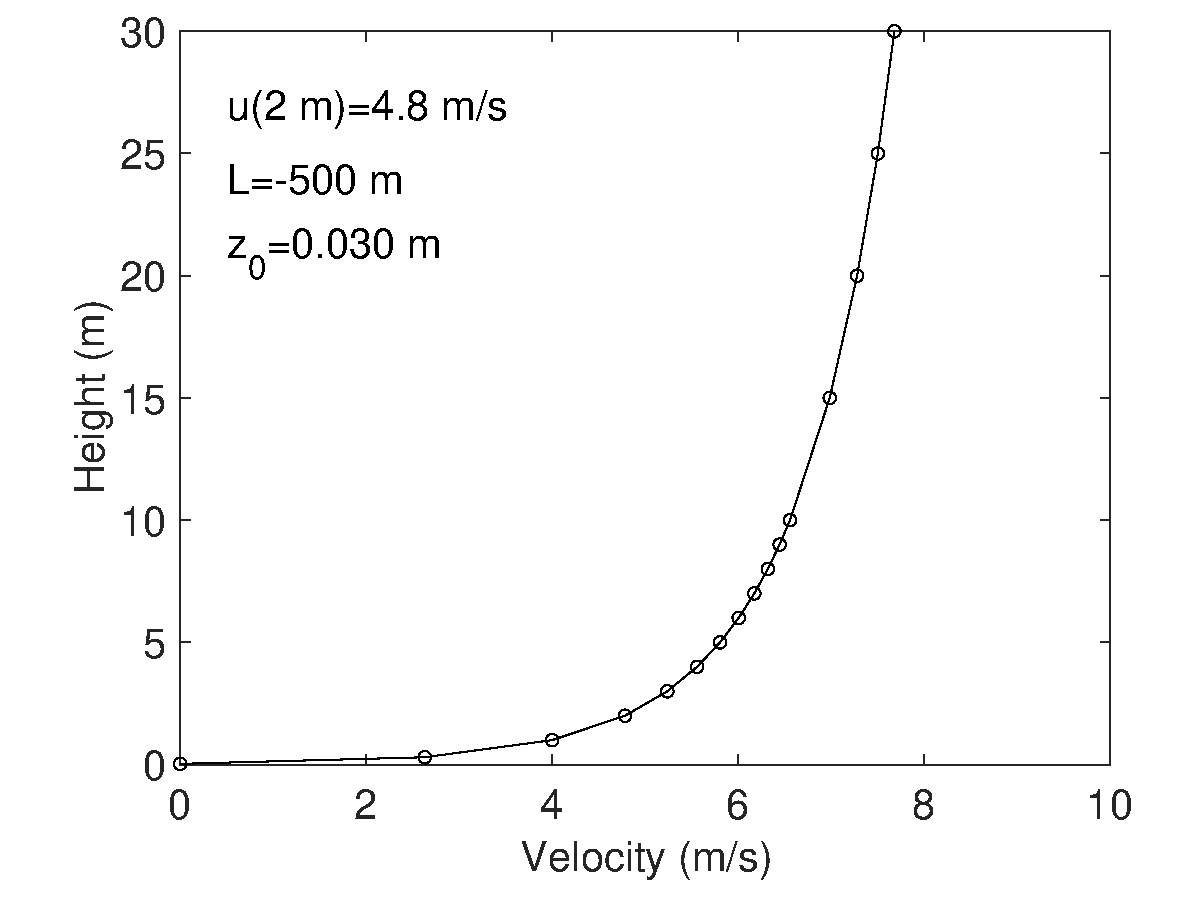
\includegraphics[width=.45\textwidth]{figures/vel_L=-500.pdf}

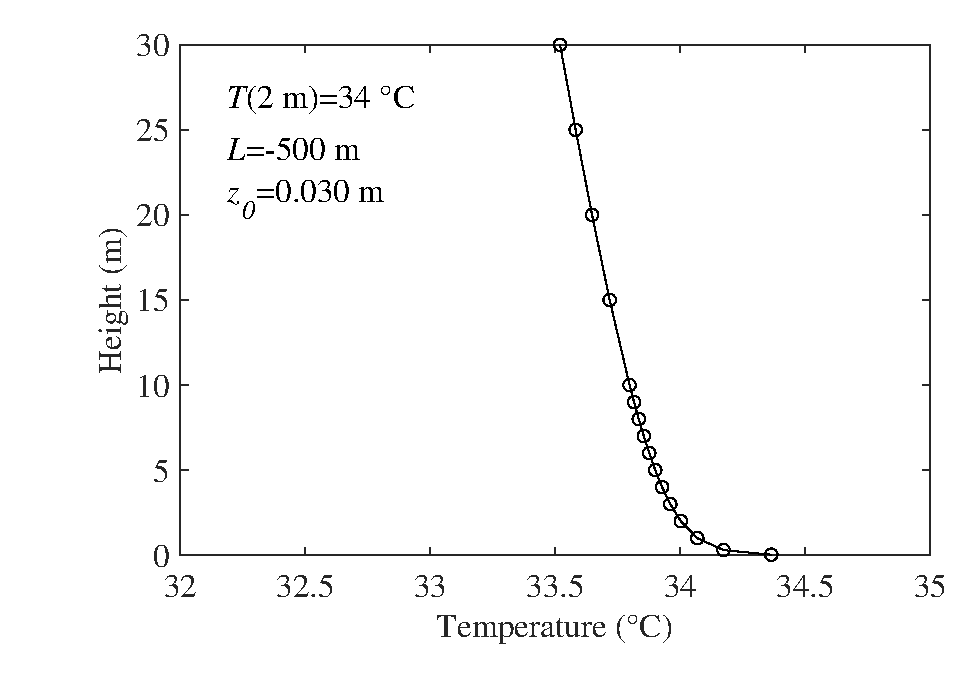
\includegraphics[width=.45\textwidth]{figures/tmp_L=-500.pdf}
\caption{Monin--Obukhov velocity and temperature profiles for inflow boundary conditions.  Here, parameters are $L=-500\;\mathrm{m}$, $z_0=0.03\;\mathrm{m}$, and~$u_r=4.8\;\mathrm{m/s}$ and $T_r=34\;^\circ\mathrm{C}$.} 
\label{fig:MOprofs}
\end{figure}

% \subsection{Turbulent Inflow Conditions}

% It is possible in FDS to superimpose synthetic turbulence on a specified inlet profile utilizing Jarrin's synthetic eddy method (SEM) \cite{Jarrin:2008}.  An example verification case is presented in Figure~\ref{fig:semprofs}.  The left image of the figure shows contours of the normal component of velocity at the inlet.  The plot on the right shows the mean and rms profiles compared to the specified inlet parameters.  The domain is 20 m in the streamwise dimension by 12 m in the spanwise by 13 m in height.  In The turbulence intensity is set to 10 \% and the turbulence integral length scale is set to 3 m.  The specified MO parameters are $L=-667\;\mathrm{m}$, $z_0=0.022\;\mathrm{m}$, and $u_r=10\;\mathrm{m/s}$ and $T_r=20\;^\circ\mathrm{C}$ at reference height of 10 m.  The simulation runs for 60 seconds with statistics collected over the last 30 seconds.  The lateral, top, and downstream boundaries are set to ``open'' pressure boundaries as discussed in the next section.

% \begin{figure}[ht]
% %\centering
% 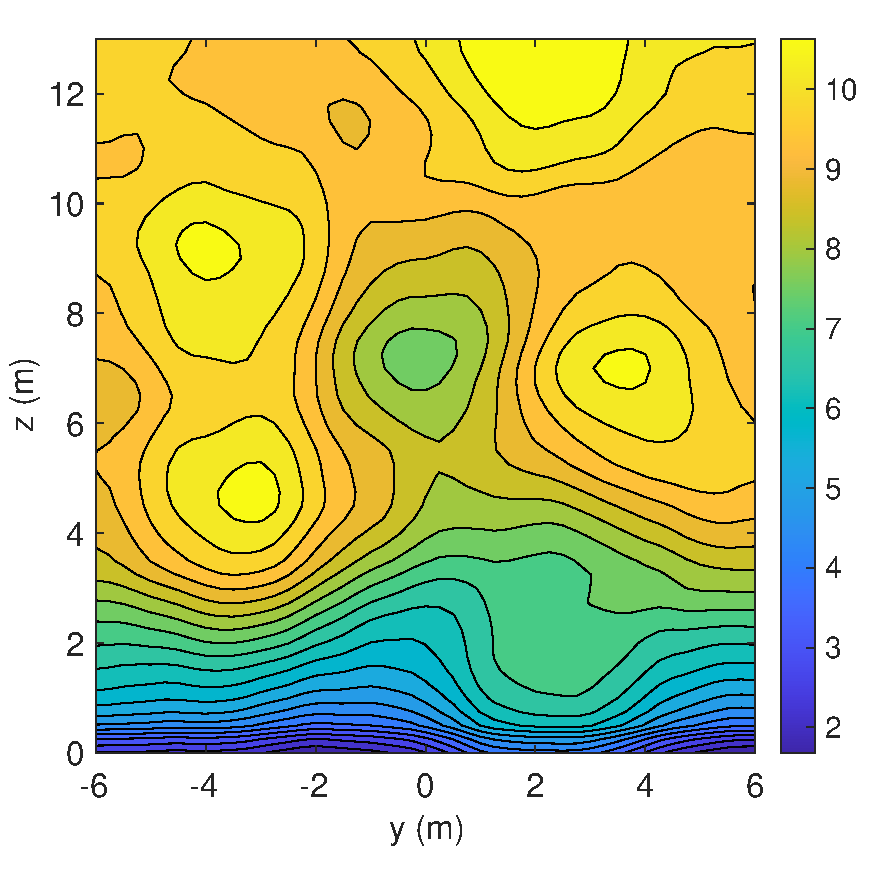
\includegraphics[width=0.5\textwidth,valign=c]{figures/sem_open_wind_contours.pdf}
% 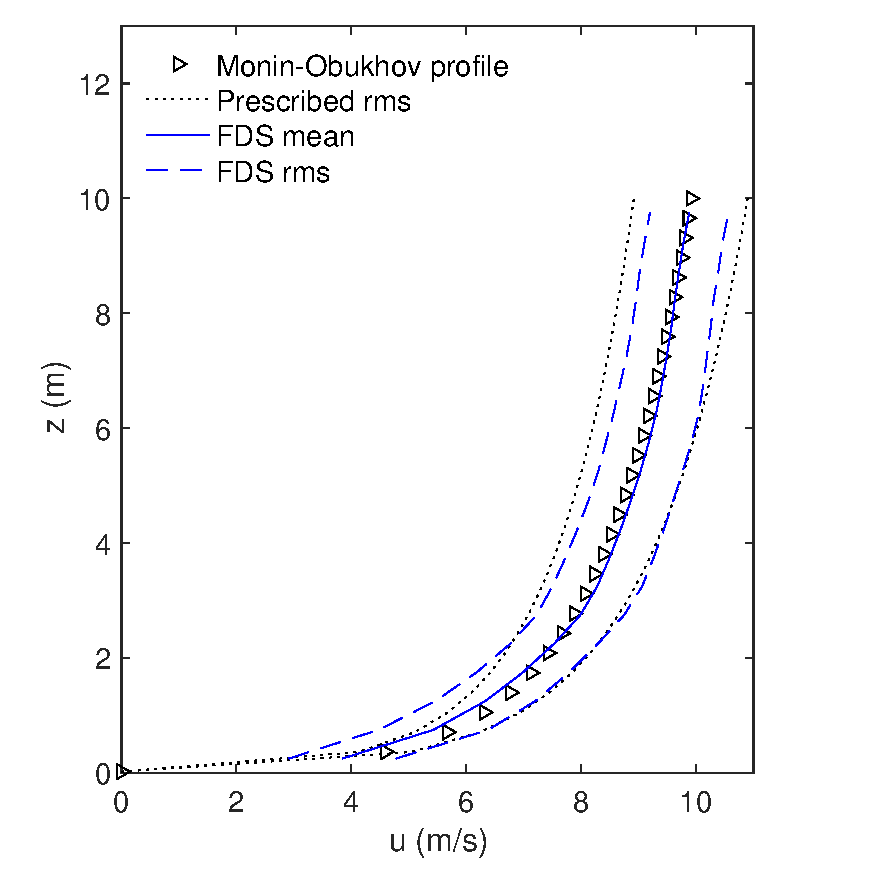
\includegraphics[width=0.48\textwidth,valign=c]{figures/sem_open_wind_u_prof.pdf}
% \caption{Example of inflow synthetic turbulence superimposed on a Monin-Obukhov boundary layer profile. Contours of the normal component of velocity at the domain inlet taken at a time midway through the simulation (left); mean and rms profiles along the inlet compared with specified profiles (right).}
% \label{fig:semprofs}
% \end{figure}

% Other approaches to imposing boundary layer turbulence are possible (e.g., \cite{Munoz-Esparza:2014}).  The cases presented later in this paper do not utilize SEM since detailed data on the turbulence statistics were not available.

\subsection{Pressure Boundary~Values}

The Poisson equation for $H$, Equation~(\ref{it:FSPoisson}), links the momentum equation with mass and energy in the low-Mach flow algorithm.  The~boundary conditions for this equation determine the inflow and outflow velocity component values.  Let $\mathbf{n}$ denote a unit normal vector pointing \emph{into} the domain.  Boundary values at an interface are denoted with a subscript ``$I$''.  Then, $\mathbf{u}_I\cdot\mathbf{n}>0$ is an inflow, and $\mathbf{u}_I\cdot\mathbf{n}<0$ is an outflow~condition.

At an inflow, the mean viscous and convective forces are generally small, and a simplified momentum equation   may be used to develop a boundary value for $H$, namely, $\partial u_i/\partial t = -\partial H/\partial x_i$. To~develop the boundary condition, let $u$ denote the $x$-component of velocity and consider an interface normal to $x$ pointing into the domain.  The~prescribed external wind field velocity component at height $z$ and time $t$ (discussed above in \mbox{Section~\ref{sec:veltmpprof}}) is denoted $u_{wind}(z,t)$.  Using a one-sided difference for $H$ and an explicit Euler approximation of the velocity time derivative, the~boundary value for $H$ may be written as
\begin{equation}
\label{eq:Hin}
H_I = H_{I\pm\frac{1}{2}}^n \pm \frac{\Delta x}{2}\left[\frac{u_{wind,I}(z,t) - u_I^n}{\Delta t}\right] \quad \mbox{if} \quad \mathbf{u}_I\cdot\mathbf{n}>0.
\end{equation}

At an outflow boundary, $H$ is set equal to the local kinetic energy per unit mass from the cell just upwind of the boundary:
\begin{equation}
\label{eq:Hout}
H_I = \frac{1}{2}(\bar{u}^n \bar{u}^n + \bar{v}^n \bar{v}^n + \bar{w}^n \bar{w}^n)_{I\pm\frac{1}{2}} \quad \mbox{if} \quad \mathbf{u}_I\cdot\mathbf{n}<=0.
\end{equation}

The overbar on the velocity components denotes a linear interpolation of the primitive staggered component values to the cell~center.

\section{Numerical~Experiments} \label{sec:numexp}
\unskip


\subsection{Flat Terrain Fire~Spread}  \label{sec:simexp}

In July and August of 1986, the~Commonwealth Scientific and Industrial Research Organisation (CSIRO) of Australia conducted controlled grassland fire experiments near Darwin, Northern Territory~\cite{Cheney:IJWF1993}. July and August are in the middle of the dry season when the grasses are fully cured (dried) and the weather is warm and dry. The~experiments were conducted on flat plots measuring 100~m by 100~m, 200~m by 200~m, or~200~m by 300~m. Two cases have been simulated. Case~C064 was conducted on a 100~m by 100~m plot of kerosene grass ({\it Eriachne burkittii}); Case~F19 was conducted on a 200~m by 200~m plot of kangaroo grass ({\it Themeda australis}).

Two of these experiments were originally simulated with FDS by Mell~et~al.~\cite{Mell:IJWF2007} using a form of the Boundary Fuel Model. Now these two experiments are also simulated using the Lagrangian Particle Model and the Level Set Model. The~level set simulations of Case~C064 use fuel index 1 (Short Grass) and for Case~F19, fuel index 3 (Tall Grass)~\cite{Rothermel:1972,Albini:1976}.

Measured bulk properties of the grasses burned in the two experiments are listed in Table~\ref{Properties_Grasses}. Properties that were not measured are listed in Table~\ref{Assumed_Properties_Grasses}. These assumed properties are typically for wood or cellulosic fuels. The~moisture is modeled as water. The~grass is assumed to be composed primarily of~cellulose.

\begin{specialtable}[H] 
\caption[Measured properties for the CSIRO Grassland Fire cases]{Measured properties for the CSIRO Grassland Fire cases~\cite{Cheney:IJWF1993}.}
\label{Properties_Grasses}
\setlength{\cellWidtha}{\columnwidth/4-2\tabcolsep+0.0in}
\setlength{\cellWidthb}{\columnwidth/4-2\tabcolsep+0.0in}
\setlength{\cellWidthc}{\columnwidth/4-2\tabcolsep+0.0in}
\setlength{\cellWidthc}{\columnwidth/4-2\tabcolsep+0.0in}
\scalebox{1}[1]{\begin{tabularx}{\columnwidth}{>{\PreserveBackslash\raggedright}m{5cm}>{\PreserveBackslash\centering}m{2cm}>{\PreserveBackslash\centering}m{2.5cm}>{\PreserveBackslash\centering}m{3cm}}
\toprule
\textbf{Property}                        & \textbf{Units}        & \textbf{Case C064} & \textbf{Case F19}    \\ \midrule 
Wind Speed                      & m/s          & 4.6       & 4.8         \\ \midrule
Ambient Temperature             & $^\circ$C    & 32.       & 34          \\ \midrule
Surface Area to Volume Ratio    & m$^{-1}$     & 9770      & 12240       \\ \midrule
Grass Height                    & m            & 0.21      & 0.51        \\ \midrule
Bulk Mass per Unit Area         & kg/m$^2$     & 0.283     & 0.313       \\ \midrule
Moisture Fraction               & \%           & 6.3       & 5.8         \\ \midrule
Measured RoS                    & m/s          & 1.2       & 1.5         \\ \midrule
Calc'd RoS, Particle Method (0.25 m, 0.5 m, 1.0 m resolution) 
                                & m/s          & 1.1, 1.2, 1.2   & 1.4, 1.3, 1.4          \\ \midrule
Calc'd RoS, Boundary Fuel Method (0.25 m, 0.5 m, 1.0 m resolution) 
                                & m/s          & 1.3, 1.3, 1.3   & 1.5, 1.4, 1.7          \\ \midrule
Calc'd RoS, Level Set Method (5 m, 10 m, 20 m resolution) 
                                & m/s          & 0.5, 0.6, 0.6   & 1.0, 1.1, 1.2          \\ \bottomrule
\end{tabularx}}
\end{specialtable}

Snapshots of the Lagrangian particle simulation of Case~F19 compared to photographs of the experiment are shown in Figure~\ref{F19}. The~plot of grass is 200~m by 200~m, and the computational domain is 240~m by 240~m by 20~m high. The~grid cells are 0.5~m cubes. The~domain is subdivided into 36 individual meshes and run in parallel. A~blade of grass is represented by a single cylindrically shaped particle within a grid cell. The~radius of the cylinder is derived from the measured surface area to volume ratio of the grass. Each simulated blade of grass represents many more actual blades of grass. The~weighting factor is determined from the measured bulk mass per unit area. The~fires in the experiments were ignited by two field workers carrying drip torches walking in opposite directions along the upwind boundary of the plot (the red strip in Figure~\ref{F19}). In~FDS, this action was modeled using a specified spread rate along the~strip.




 


% start a new page without indent 4.6cm
%\clearpage
\end{paracol}
\nointerlineskip
\begin{figure}[H]
\widefigure
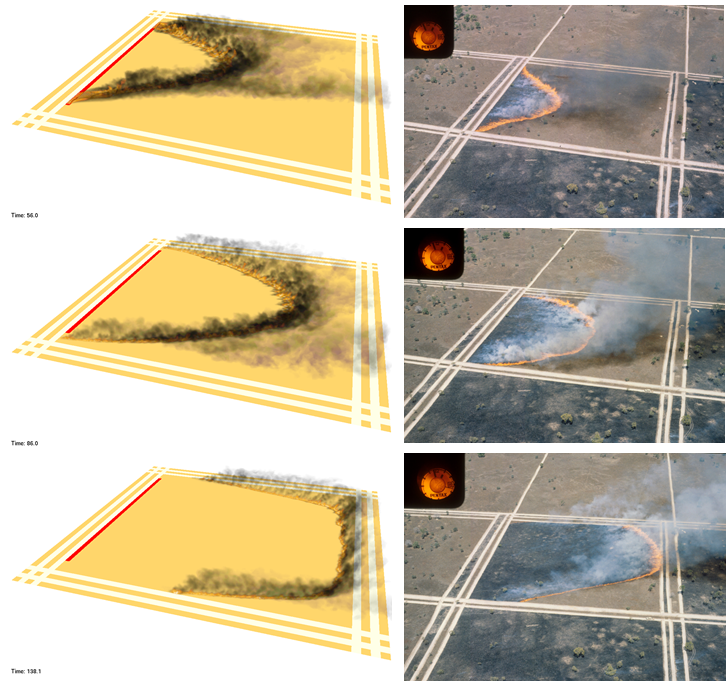
\includegraphics[width=0.9\textwidth]{figures/F19_collage.png}
\caption{Photographs of the experiment and snapshots of the simulation (medium resolution Particle Model) of CSIRO Grassland Fire F19, 56~s, 86~s, and~138~s following~ignition.}
\label{F19}
\end{figure}
\begin{paracol}{2}
%\linenumbers
\switchcolumn







The simulations were conducted with the three different fire spread models, and~each case was run with three levels of spatial resolution. The~simulations using the Particle and Boundary Fuel Models were run with cubic grid cells that were 0.25~m, 0.5~m, and~1~m on a side. The~simulations using the Level Set Model were run with cells of 5~m, 10~m, and~20~m. The~predicted rates of spread for the two cases are listed in \mbox{Table~\ref{Properties_Grasses}} and shown graphically in Figure~\ref{CSIRO}. For~these simulations, the~rate of spread predicted by the Particle and Boundary Fuel Models are comparable to the measured rate of spread, while the level set method under-predicts the RoS. The~under-prediction by the level set simulations is a consequence of the limitations of the Rothermel model, which is based on empirical relations largely derived from laboratory-scale experiments. It is well-known that practical application of the Rothermel model often requires calibration for the case of interest~\cite{Arca_2007}. The~use of the Rothermel for the head fire spread rate in surface vegetation in FDS is to be viewed as a placeholder that is in-line with other CFD-based models. If~the observed head fire rate of spread for the F19 and C064 experiments is used in FDS, \mbox{then good} agreement with the observed fire perimeter is obtained (not shown). \mbox{Further work} is needed to develop rate-of-spread models appropriate for use with the Level Set Model (e.g.,~\cite{Mell:FBFC2019}).


 \begin{specialtable}[H]
\caption[Assumed properties for dry grass and soil]{Assumed properties for various types of dried grass and soil. Note that the Pyrolysis Temperature is taken to be the temperature at which the mass loss rate peaks in the TGA experiments of Morvan and Dupuy~\cite{Morvan:CF2004}.}
\setlength{\tabcolsep}{4.1mm} 
\label{Assumed_Properties_Grasses}
\begin{tabular}{lccc}
\toprule
\textbf{Property}                        & \textbf{Units}                 & \textbf{Value}                     & \textbf{Reference}                             \\ \midrule 
Chemical Composition            & --                    & C$_6$H$_{10}$O$_5$        & Assumption                            \\ \midrule
Heat of Combustion              & kJ/kg                 & 15600                     & \cite{Susott:FS1982}                  \\ \midrule
Soot Yield                      & kg/kg                 & 0.015                     & \cite{SFPE:Tewarson}                  \\ \midrule
Char Yield                      & kg/kg                 & 0.2                       & \cite{Susott:FS1982}                  \\ \midrule
Specific Heat                   & kJ/(kg$\cdot$K)       & 1.5                       & Various sources                       \\ \midrule
Conductivity                    & W/(m$\cdot$K)         & 0.1                       & Assumption                            \\ \midrule
Density                         & kg/m$^3$              & 512                       & \cite{Rothermel:1972}                 \\ \midrule
Heat of Pyrolysis               & kJ/kg                 & 418                       & \cite{Morvan:CF2004}                  \\ \midrule
Pyrolyis Temperature            & $^\circ$C             & 200                       & \cite{Morvan:CF2004}                  \\ \midrule 
Obukhov Length                  & m                     & -500                      & Assumption                            \\ \midrule
Aerodynamic Roughness Length    & m                     & 0.03                      & Assumption                            \\ \midrule
Drag Coefficient                & --                    & 2.8                       & \cite{Falkenstein-Smith:2018}         \\ \midrule 
Soil Specific Heat              & kJ/(kg$\cdot$K)       & 2.0                       & \cite{Farouki:1981}                   \\ \midrule
Soil Conductivity               & W/(m$\cdot$K)         & 0.25                      & \cite{Farouki:1981}                   \\ \midrule
Soil Density                    & kg/m$^3$              & 1300                      & \cite{Farouki:1981}                   \\ \bottomrule

\end{tabular}
\end{specialtable}

Figure~\ref{fig:CaseF19_contours} shows contours of heat release rates near the surface compared to the observed flame front for the high-resolution (0.25 m) Particle Model.  These contours may be compared to the head fire spread rates at the top of Figure~\ref{CSIRO}.  Case F19 contours are shown on the right, and may be compared to the flame images in Figure~\ref{F19}.  These results show some improvement to the flank fire spread rates compared to previous simulations with FDS conducted by Mell~et~al.~in 2007~\cite{Mell:IJWF2007}.

However, it is difficult to compare the present results with those from~\cite{Mell:IJWF2007}. The~underlying numerical model, FDS, has undergone a major revision over the past decade, changing the basic finite-difference scheme, boundary conditions, drag modeling, and~so on, and~the vegetation-specific models have changed as well, most notably the charring reaction. In~addition, the~amount of information about the grasses and field conditions is limited, and~the thermal and kinetic parameters gleaned from various sources are generally average values over a wide range of vegetation types. A~sensitivity study~\cite{McGrattan:CI2017} for the particle model simulations reveals that near-surface wind speed has the most direct effect on the rate of spread (RoS), and~the combined effect of the dozens of thermal, \mbox{kinetic, and~numerical} parameters would certainly explain the difference in RoS between the 2007 results and those of this~study. 



% start a new page without indent 4.6cm
%\clearpage
\end{paracol}
\nointerlineskip
\begin{figure}[H]
\widefigure
\begin{tabular*}{\textwidth}{l@{\extracolsep{\fill}}r}
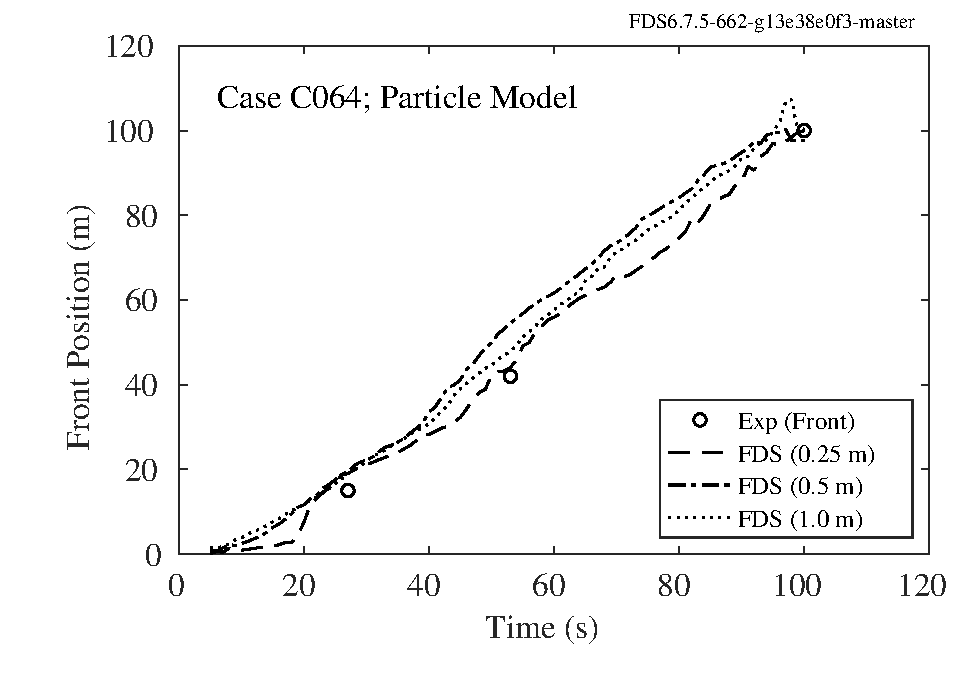
\includegraphics[height=2.2in]{figures/Case_C064} &
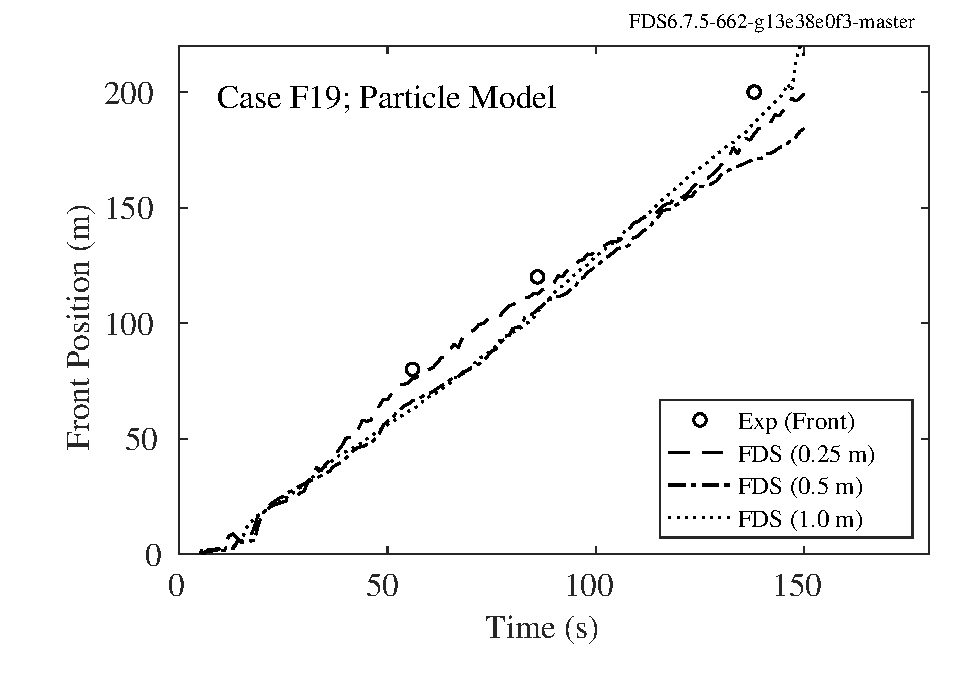
\includegraphics[height=2.2in]{figures/Case_F19} \\
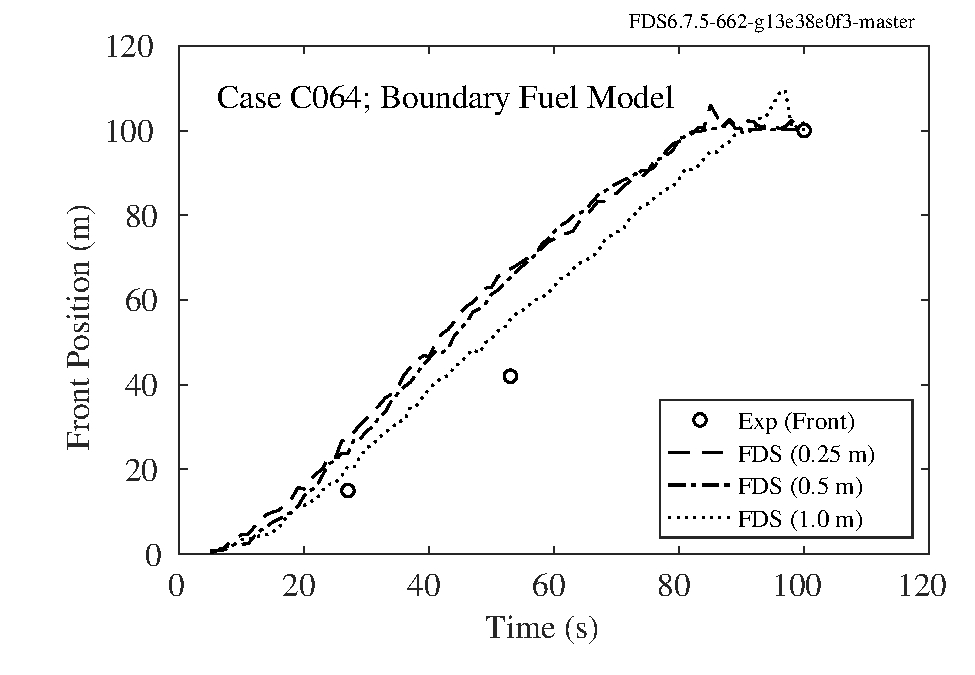
\includegraphics[height=2.2in]{figures/Case_C064_BFM} &
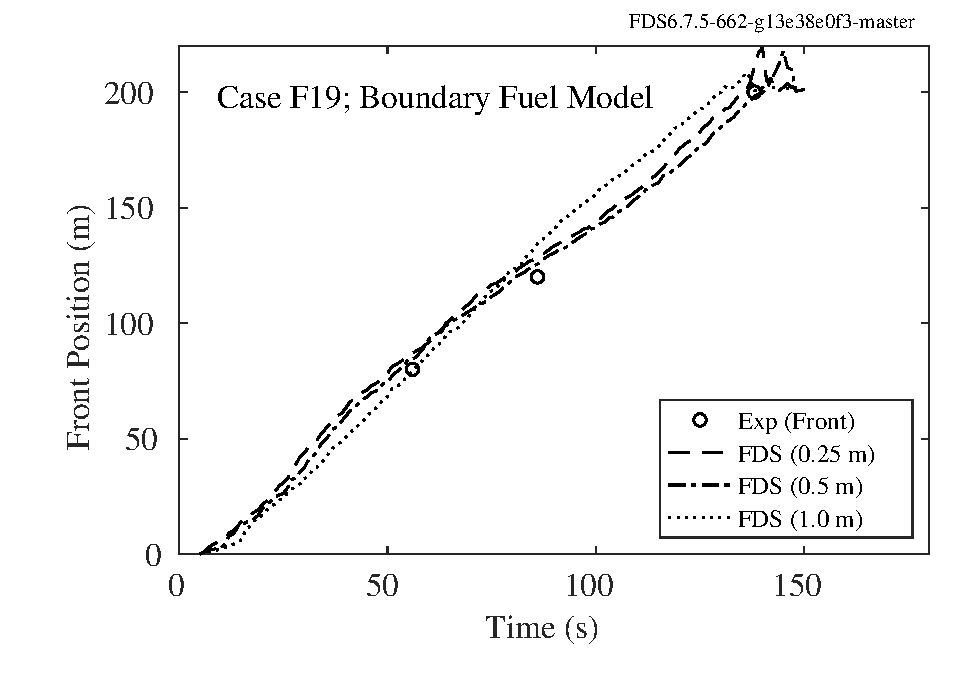
\includegraphics[height=2.2in]{figures/Case_F19_BFM} \\
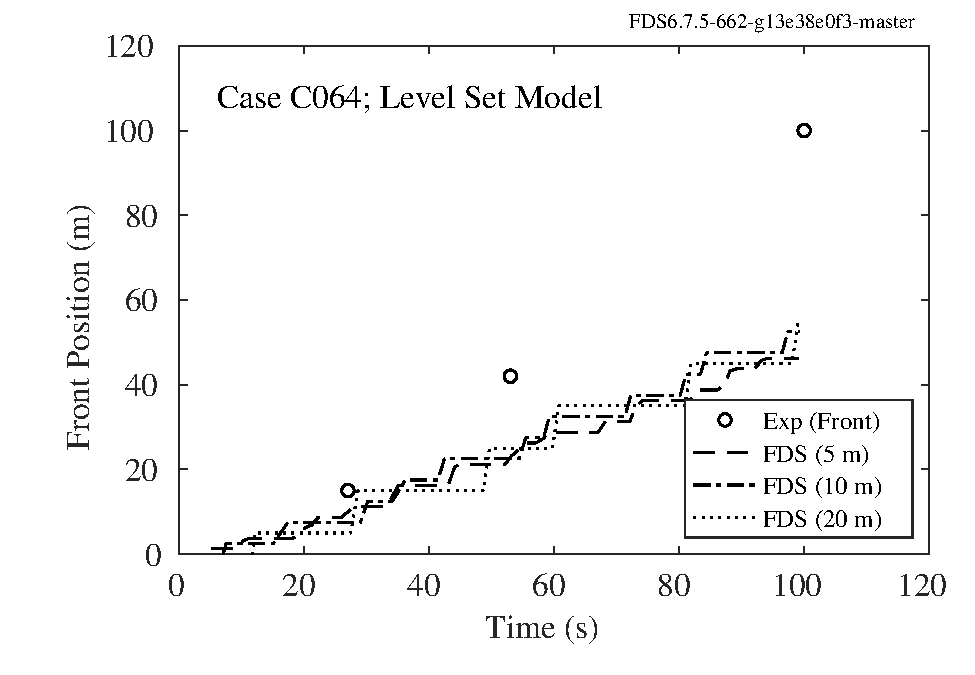
\includegraphics[height=2.2in]{figures/Case_C064_LS}  &
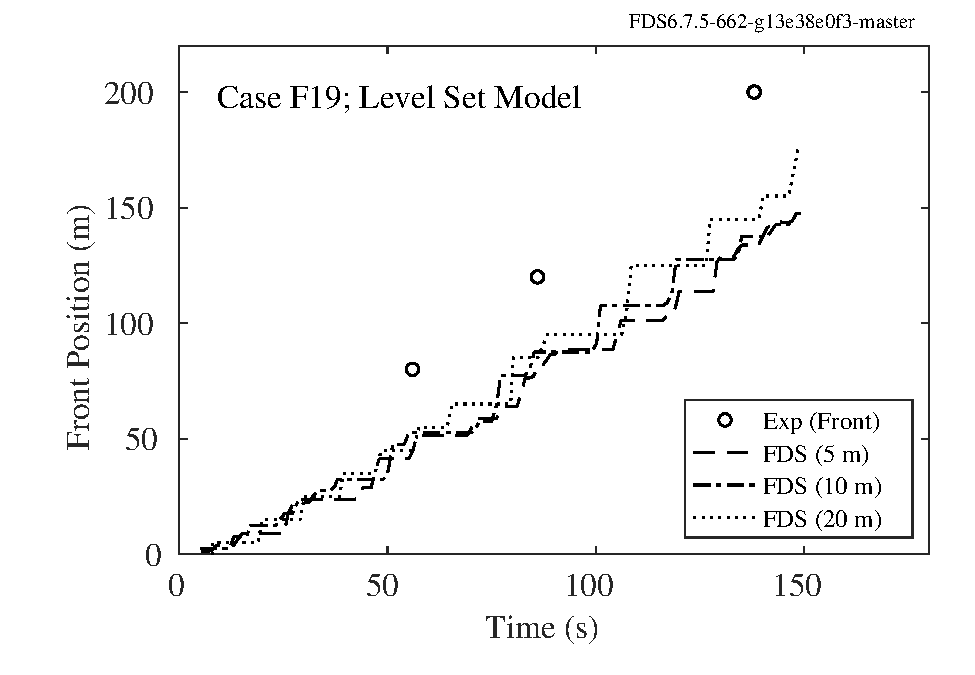
\includegraphics[height=2.2in]{figures/Case_F19_LS}
\end{tabular*}
\caption{Comparison of the measured and predicted fire front position for the CSIRO Grassland Fires using three different methods of fire~spread.}
\label{CSIRO}
\end{figure}
\begin{paracol}{2}
%\linenumbers
\switchcolumn



% start a new page without indent 4.6cm
\clearpage
\end{paracol}
\nointerlineskip
\begin{figure}[H]
\vspace{-18pt}
\widefigure
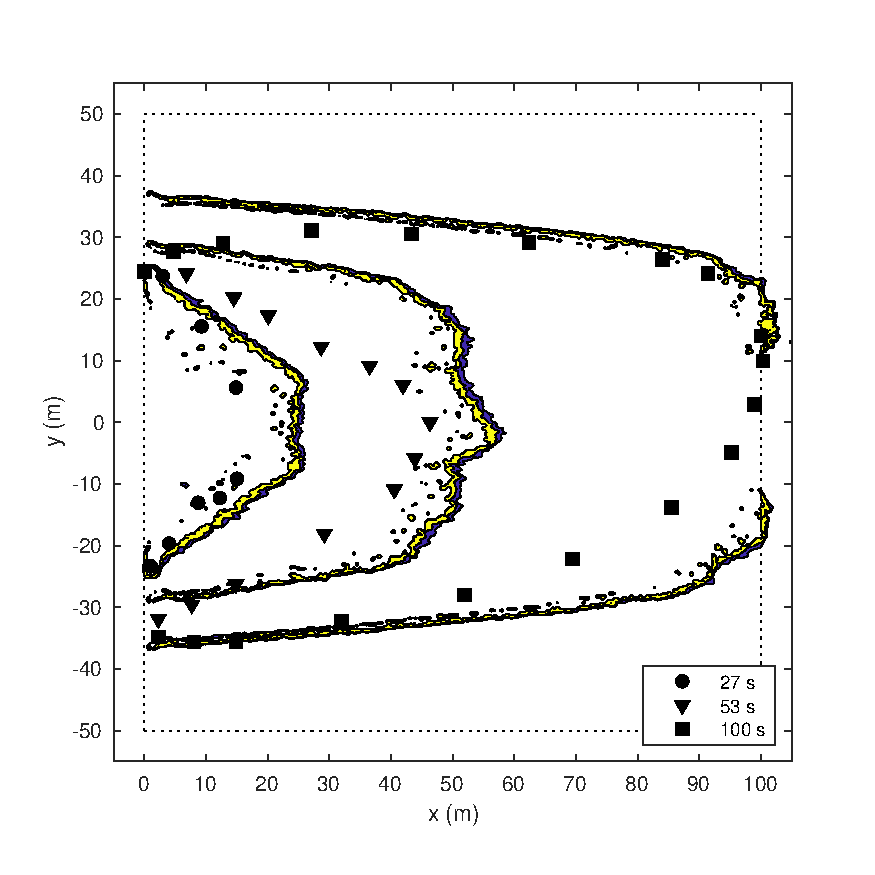
\includegraphics[width=0.49\textwidth]{figures/Case_C064_flame_position.pdf}
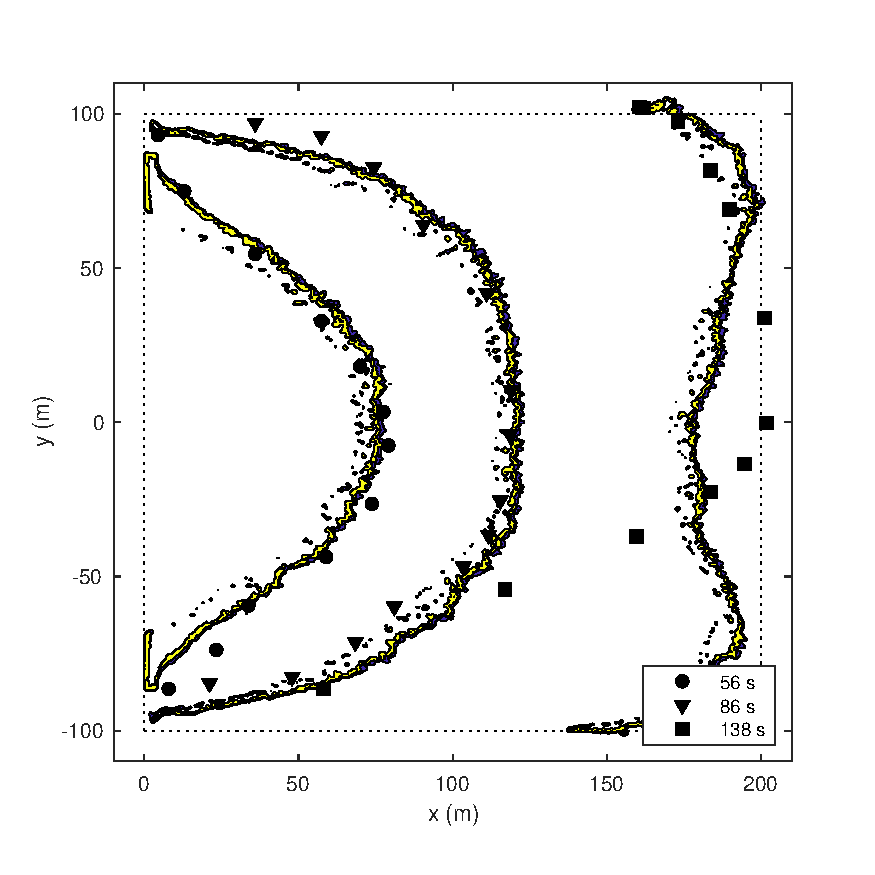
\includegraphics[width=0.49\textwidth]{figures/Case_F19_flame_position.pdf}
\vspace{-6pt}
\caption{Contours of heat release rate in a plane near the surface from the fine resolution (0.25 m) Particle Model compared to observations of CSIRO Grassland Fires C064 (\textbf{left}) and F19 (\textbf{right}).}
\label{fig:CaseF19_contours}
\end{figure}
\begin{paracol}{2}
%\linenumbers
\switchcolumn



\subsection{Complex Terrain Fire~Spread}  
\label{sec:cogo}

This section presents an example of the methodologies discussed in the paper. It is notable because it considers an actual fire that occurred in the wildland–urban interface (WUI), which presents a challenge for a fire spread model because the surface vegetation is mixed with the built~environment.

At approximately 23:00 (local time) on  25 March 2019, a~wildfire started in the seaside town of Cogoleto, near~Genoa, Italy. Strong winds, gusting up to 100~km/h from the north, spread the fire from its ignition point towards the sea. The~fire was caused by a faulty power line on a ridge above the town. Several houses were destroyed, and hundreds of residents had to be evacuated. The~burnt region measured over 1~km from the origin to the farthest point. The~fire burned overnight and into the next day. Up~to 70 firefighters worked at the scene, with~help from helicopters and fire hydrants. Suppression efforts were directed towards stopping the fire spread into the coastal town of~Cogoleto.

Shown in Figure~\ref{Cogoleto_satellite} are the results of a level set simulation of the fire superimposed on a satellite photograph of the area and the outline of the extent of the actual fire. The~computational domain was assembled using an open-source, Geographic Information System (GIS) program called QGIS~\cite{QGIS}, extended by the qgis2fds~\cite{qgis2fds} plugin. The~open-source qgis2fds plugin was specifically developed in the framework of the WUIFI-21 project for facilitating the use of geographical data for forest fire simulation and smoke pollutants dispersion in~FDS (WUIFI-21: {\it High-fidelity computational fluid dynamics modeling of forest fires for wildland–urban Interface communities resilience and protection} is an~Italy–US research project financed by the Italian Ministry of Foreign Affairs and International Cooperation).

The wind speed and direction are based on a single weather station near the point of ignition. Winds recorded were found to be predominantly coming from the north, with magnitudes that ranged from 20~m/s during the night and diminishing to 5~m/s towards the morning hours. The~vegetation type was provided by a database maintained at the International Centre on Environmental Monitoring (CIMA) %The journal does not allow footnotes, and the footnotes are unified into the main text. Please confirm.
Research Foundation, derived from regional forest management maps. In~the simulation, the~single-point wind data were taken as the prevailing wind, and~the local wind field was obtained via  CFD computation. The~fire was simulated based on the position of the level set front; that is, when the front arrived at a given location, a~fire was ignited and burned for a duration of time consistent with the specified fuel loading of that particular point on the~map. 

% start a new page without indent 4.6cm
%\clearpage
\end{paracol}
\nointerlineskip
\begin{figure}[H]
\vspace{-12pt}
\widefigure
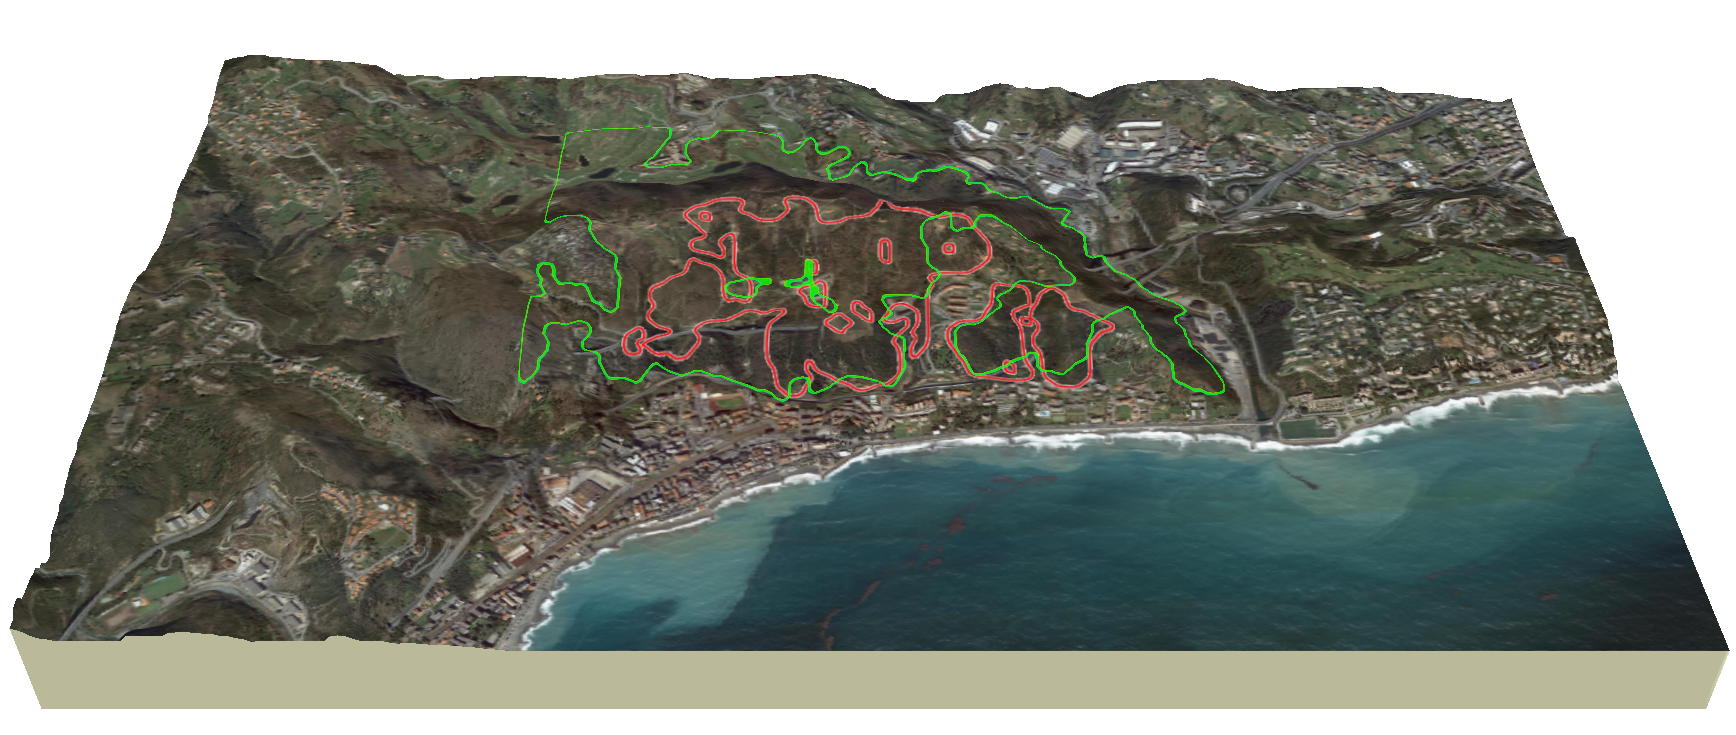
\includegraphics[width=0.9\textwidth]{figures/cogoleto_fire_2019_ls4_1000.png}
\caption{Satellite photograph of the region where the Cogoleto Fire occurred. The~area outlined in red is the extent of the actual fire; green is the~simulation.}
\label{Cogoleto_satellite}
\end{figure}
\begin{paracol}{2}
%\linenumbers
\switchcolumn




The extent of the simulated fire, shown in green in Figure~\ref{Cogoleto_satellite}, is greater than that of the actual fire, shown in red. This is not surprising, given that the simulation does not include suppression and the rate of spread of the level set front is determined based on vegetation that may not exactly resemble that of this particular region. It is important to note that for the level set method, a~fire break created by first responders can be modeled as a region declared as "non-combustible". The 13 Rothermel fuel types have been supplemented by areas such as water, pavement, and~other non-combustibles. The~fire-front determined by the level set calculation is stopped by the non-combustible area, highlighting the challenge in simulating firebrand spot ignitions that were reported by first responders at the~scene.

The simulation results have been compared with those obtained from the CIMA Propagator~\cite{Trucchia:2020}, an~experimental propagation model that has provided several European civil protection organizations with real-time fire predictions since 2009. The~model has been implemented by the CIMA Foundation, and its propagation model is based on stochastic cellular~automata.

The two models produce a qualitatively similar patterns of fire spread, mainly because the vicinity of the fire has numerous areas that are considered ``non-combustible',' that is, devoid of vegetation or structures. This points out the problem of ``validating'' wildfire models. The~simulations of the flat terrain grassland fire experiments described in the previous section match the observed fire behavior fairly well, but~in those cases, the~vegetation is uniform and fairly well-described in terms of its mass loading and geometrical characteristics, the~terrain is flat and of relatively small area, the~wind is steady, and~the experiment lasts a few minutes. In~a real fire, none of this will be true. The~detailed physics of the fire are not resolvable on a relatively coarse grid, the~vegetation is heterogeneous, sparse, and~sometimes unknown, the~weather conditions are varying, there are suppression efforts with water and the setting of backfires, and~the fires can burn for~days.

All of this raises the question as to what level of physical fidelity ought to be required in these models. The~strategy that has been adopted in FDS is to accommodate simulation options ranging from a level set calculation of fire spread over tens of kilometers that can be run in minutes, similar to models like FARSITE developed by the US Forest Service, \mbox{all the} way to detailed simulations of fire spread at sub-meter resolution for relatively short time-periods (minutes to hours) and small areas (tens of hectares). As~was the case for models developed for building fires 30 years ago, it is not clear at the moment exactly how these wildland fire models will be used in the future. The~best strategy is to advance the various modeling options until a clear path forward becomes~apparent.


\section{Summary} \label{sec:summary}

The numerical methods described in this paper span the range of length scales from tens of centimeters to tens of kilometers. Obviously, these techniques support differing descriptions of the underlying fire physics, but~all can be embedded within the same code base. This allows researchers to combine the different techniques in ways that were not possible when separate codes were maintained by separate organizations. With~FDS, \mbox{one can} simulate 24 hours of fire spread in minutes of computation time using the level set function and a wind field that varies only temporally, not spatially, with~no fire–atmospheric coupling. At~the same time, using the same set of input parameters, one can simulate the fire at far greater resolutions with much greater physical fidelity, albeit for shorter time-periods and spatial~extent.

\vspace{6pt}

\authorcontributions{Conceptualization, M.V.; Data curation, R.M.; Investigation, K.M. and W.M.; Software, E.G. and P.F.; Visualization, G.F.}

\funding{This work was partially funded by the Risk Reduction in Communities Program at NIST. W.M. acknowledges support from the Strategic Environmental Research and Development Program (SERDP) Grant RC19-1132.} 

\dataavailability{The Fire Dynamics Simulator is an open-source computational fluids dynamics code available at \href{https://github.com/firemodels/fds}{https://github.com/firemodels/fds}. The input files for the CSIRO wildfire spread calculations are also kept within this repository.}

 
\conflictsofinterest{The authors declare no conflict of interest.}


\end{paracol}
\reftitle{References}


%\bibliography{Review_Process/FDS_refs,Review_Process/LOFM_Workshop_References,Review_Process/Vanella_Article_Atmosphere_2020}

\begin{thebibliography}{999}

\bibitem[Thomas \em{et~al.}(2017)Thomas, Butry, Gilbert, Webb, and
  Fung]{thomas_2017}
Thomas, D.; Butry, D.; Gilbert, S.; Webb, D.; Fung, J.
\newblock The Costs and Losses of Wildfires: A Literature Review.
\newblock Special Publication NIST SP - 1215, National Institute of Standards
  and Technology, Gaithersburg, Mayland,  2017.
\newblock
  \href{https://www.nist.gov/publications/costs-and-losses-wildfires}{https://www.nist.gov/publications/costs-and-losses-wildfires} (accessed on 05/02/2021).

\bibitem[McDermott \em{et~al.}(2019)McDermott, Bryner, and
  Heintz]{mcdermott_2019}
McDermott, R.; Bryner, N.; Heintz, J.
\newblock Large Outdoor Fire Modeling (LOFM) Workshop Summary Report.
\newblock Special Publication NIST SP - 1245, National Institute of Standards
  and Technology, Gaithersburg, Mayland,  2019.
\newblock
  \href{https://www.nist.gov/publications/large-outdoor-fire-modeling-lofm-workshop-summary-report}{https://www.nist.gov/publications/large-outdoor-fire-modeling-lofm-workshop-summary-report} (accessed on 05/02/2021).

\bibitem[Richards \em{et~al.}(2020)Richards, Brew, and Smith]{richards_2020}
Richards, L.; Brew, N.; Smith, L.
\newblock 2019–20 Australian bushfires—frequently asked questions: a quick
  guide.
\newblock Research Paper Series 2019-20, ISSN 2203-5249, Parliament of
  Australia, Canberra, Australia,  2020.
\newblock
  \href{https://parlinfo.aph.gov.au/parlInfo/download/library/prspub/7234762/upload\_binary/7234762.pdf}{https://parlinfo.aph.gov.au/parlInfo/download/library/prspub/7234762/upload\_binary/7234762.pdf} (accessed on 05/02/2021).

\bibitem[Papadopoulos and Niovi~Pavlidou(2011)]{Papadopoulos_2011}
Papadopoulos, G.D.; Niovi~Pavlidou, F.
\newblock A review of a new generation of wildfire–atmosphere modeling.
\newblock {\em IEEE Systems Journal} {\bf 2011}, {\em 5},~233--243.

\bibitem[Bakhshaii and Johnson(2019)]{Bakhshaii_2019}
Bakhshaii, A.; Johnson, E.
\newblock A review of a new generation of wildfire–atmosphere modeling.
\newblock {\em Canadian Journal of Forest Research} {\bf 2019}, {\em
  49},~565--574.

\bibitem[Rothermel(1972)]{Rothermel:1972}
Rothermel, R.C.
\newblock A mathematical model for predicting fire spread in wildland fuels.
\newblock Technical Report INT-115, USDA Forest Service, Ogden, Utah,  1972.
\newblock
  \href{http://www.treesearch.fs.fed.us/pubs/32533}{http://www.treesearch.fs.fed.us/pubs/32533} (accessed on 05/02/2021).

\bibitem[Anderson(1982)]{Anderson:1982}
Anderson, H.
\newblock {Aids to Determining Fuel Models for Estimating Fire Behavior}.
\newblock General Technical Report INT-122, Intermountain Forest and Range
  Experiment Station, USDA Forest Service, Ogden, Utah,  1982.
\newblock
  \href{https://www.fs.usda.gov/treesearch/pubs/6447}{https://www.fs.usda.gov/treesearch/pubs/6447} (accessed on 05/02/2021).

\bibitem[Finney(2004)]{Finney:FARSITE}
Finney, M.
\newblock {Fire Area Simulator – Model, Development and Evaluation}.
\newblock Research Paper RMRS-RP-4 Revised, United States Forest Service, Rocky
  Mountain Research Station, Missoula, Montana,  2004.
\newblock
  \href{http://www.fs.fed.us/rm/pubs/rmrs\_rp004.pdf}{http://www.fs.fed.us/rm/pubs/rmrs\_rp004.pdf} (accessed on 05/02/2021).

\bibitem[Bova \em{et~al.}(2015)Bova, Mell, and Hoffman]{Bova:IJWF2015}
Bova, A.; Mell, W.; Hoffman, C.
\newblock {A comparison of level set and marker methods for the simulation of
  wildland fire front propagation}.
\newblock {\em International Journal of Wildland Fire} {\bf 2015}, {\em
  25},~229--241.
\newblock
  \href{http://dx.doi.org/10.1071/WF13178}{http://dx.doi.org/10.1071/WF13178} (accessed on 05/02/2021).

\bibitem[McGrattan \em{et~al.}(2013)McGrattan, Hostikka, McDermott, Floyd,
  Weinschenk, and Overholt]{FDS_Users_Guide}
McGrattan, K.; Hostikka, S.; McDermott, R.; Floyd, J.; Weinschenk, C.;
  Overholt, K.
\newblock {\em {Fire Dynamics Simulator, User's Guide}}.
\newblock National Institute of Standards and Technology, Gaithersburg,
  Maryland, USA, and VTT Technical Research Centre of Finland, Espoo, Finland,
  sixth ed.,  2013.

\bibitem[Coen(2013)]{Coen:2}
Coen, J.L.
\newblock {Modeling Wildland Fires: A Description of the Coupled
  Atmosphere-Wildland Fire Environment Model (CAWFE)}.
\newblock Technical Report NCAR/TN500+STR, National Center for Atmospheric
  Research, Boulder, CO,  2013.

\bibitem[Coen and Schroeder(2015)]{Coen:2015}
Coen, J.L.; Schroeder, W.
\newblock {The High Park Fire: Coupled weather-wildland fire model simulation
  of a windstorm-driven wildfire in Colorado's Front Range}.
\newblock {\em J. Geophys. Res. Atmos.} {\bf 2015}, {\em 120},~131--146.

\bibitem[Lautenberger(2013)]{LAUTENBERGER_2013}
Lautenberger, C.
\newblock Wildland fire modeling with an Eulerian level set method and
  automated calibration.
\newblock {\em Fire Safety Journal} {\bf 2013}, {\em 62},~289 -- 298.
\newblock
  \href{https://doi.org/10.1016/j.firesaf.2013.08.014}{https://doi.org/10.1016/j.firesaf.2013.08.014} (accessed on 05/02/2021).

\bibitem[Coen \em{et~al.}(2013)Coen, Cameron, Michalakes, Patton, Riggan, and
  Yedinak]{coen_2013}
Coen, J.L.; Cameron, M.; Michalakes, J.; Patton, E.G.; Riggan, P.J.; Yedinak,
  K.M.
\newblock WRF-Fire: Coupled Weather–Wildland Fire Modeling with the Weather
  Research and Forecasting Model.
\newblock {\em Journal of Applied Meteorology and Climatology} {\bf 2013}, {\em
  52},~16--38.
\newblock
  \href{https://doi.org/10.1175/JAMC-D-12-023.1}{https://doi.org/10.1175/JAMC-D-12-023.1} (accessed on 05/02/2021).

\bibitem[Mandel \em{et~al.}(2009)Mandel, Beezley, Coen, and Kim]{Mandel:2009}
Mandel, J.; Beezley, J.D.; Coen, J.L.; Kim, M.
\newblock {Data assimilation for wildland fires: Ensemble Kalman filters in
  coupled atmosphere-surface models}.
\newblock {\em IEEE Control Systems Magazine} {\bf 2009}, {\em 9},~47–65.
\newblock
  \href{https://doi.org/10.1109/MCS.2009.932224}{https://doi.org/10.1109/MCS.2009.932224} (accessed on 05/02/2021).

\bibitem[Mandel \em{et~al.}(2011)Mandel, Beezley, and Kochanski]{Mandel:2011}
Mandel, J.; Beezley, J.D.; Kochanski, A.K.
\newblock {Coupled atmosphere-wildland fire modeling with WRF 3.3 and SFIRE
  2011}.
\newblock {\em Geosci. Model Dev.} {\bf 2011}, {\em 4},~591--610.
\newblock
  \href{https://doi.org/10.5194/gmd-4-591-2011}{https://doi.org/10.5194/gmd-4-591-2011} (accessed on 05/02/2021).

\bibitem[Mandel \em{et~al.}(2015)Mandel, Amram, Beezley, Kelman, Kochanski,
  Kondratenko, Lynn, Regev, and Vejmelka]{Mandel:2014}
Mandel, J.; Amram, S.; Beezley, J.D.; Kelman, G.; Kochanski, A.K.; Kondratenko,
  V.Y.; Lynn, B.H.; Regev, B.; Vejmelka, M.
\newblock {Recent advances and applications of WRF-SFIRE}.
\newblock {\em Nat. Hazards Earth Syst. Sci.} {\bf 2015}, {\em 14},~2829--2845.
\newblock
  \href{https://doi.org/10.5194/nhess-14-2829-2014}{https://doi.org/10.5194/nhess-14-2829-2014} (accessed on 05/02/2021).

\bibitem[Kochanski \em{et~al.}(2016)Kochanski, Jenkins, Yedinak, Mandel,
  Beezley, and Lamb]{Kochanski:2016}
Kochanski, A.K.; Jenkins, M.A.; Yedinak, K.; Mandel, J.; Beezley, J.; Lamb, B.
\newblock {Toward an integrated system for fire, smoke, and air quality
  simulations}.
\newblock {\em Int. J. Wildland Fire} {\bf 2016}, {\em 25},~534–546.
\newblock
  \href{https://doi.org/10.1071/WF14074}{https://doi.org/10.1071/WF14074} (accessed on 05/02/2021).

\bibitem[Sethian(1999)]{Sethian:1999}
Sethian, J.A.
\newblock {\em Level Set Methods and Fast Marching Methods: Evolving Interfaces
  in Computational Geometry, Fluid Mechanics, Computer Vision, and Materials
  Science}; Cambridge,  1999.

\bibitem[Osher and Fedkiw(2006)]{Osher:2006}
Osher, S.; Fedkiw, R.
\newblock {\em Level Set Methods and Dynamic Implicit Surfaces}; Springer,
  2006.

\bibitem[Mell \em{et~al.}(2007)Mell, Jenkins, Gould, and Cheney]{Mell:IJWF2007}
Mell, W.; Jenkins, M.; Gould, J.; Cheney, P.
\newblock {A physics-based approach to modelling grassland fires}.
\newblock {\em International Journal of Wildland Fire} {\bf 2007}, {\em
  16},~1--22.

\bibitem[Linn \em{et~al.}(2007)Linn, Winterkamp, Edminster, Colman, and
  Smith]{Linn:2007}
Linn, R.; Winterkamp, J.; Edminster, C.; Colman, J.J.; Smith, W.S.
\newblock {Coupled influences of topography and wind on wildland fire
  behaviour}.
\newblock {\em Int. J. Wildland Fire} {\bf 2007}, {\em 16},~183--195.

\bibitem[Arca \em{et~al.}(2019)Arca, G., M., M., and P.]{Arca_2019}
Arca, B.; G., T.; M., C.; M., S.; P., D.
\newblock A web-based wildfire simulator for operational applications.
\newblock {\em International Journal of Wildland Fire} {\bf 2019}, {\em
  28},~99--112.

\bibitem[Rehm and Baum(1978)]{Rehm:1}
Rehm, R.; Baum, H.
\newblock {The Equations of Motion for Thermally Driven, Buoyant Flows}.
\newblock {\em Journal of Research of the NBS} {\bf 1978}, {\em 83},~297--308.

\bibitem[McDermott and Floyd(2015)]{McDermott:2015}
McDermott, R.; Floyd, J.
\newblock {Enforcing realizability in explicit multi-component species
  transport}.
\newblock {\em Fire Safety Journal} {\bf 2015}, {\em 78},~180--187.

\bibitem[McDermott(2014)]{mcdermo_2014}
McDermott, R.J.
\newblock A velocity divergence constraint for large-eddy simulation of
  low-Mach flows.
\newblock {\em Journal of Computational Physics} {\bf 2014}, {\em
  274},~413--431.
\newblock
  \href{http://dx.doi.org/10.1016/j.jcp.2014.06.019}{http://dx.doi.org/10.1016/j.jcp.2014.06.019} (accessed on 05/02/2021).

\bibitem[Pope(2000)]{Pope:2000}
Pope, S.B.
\newblock {\em Turbulent Flows}; Cambridge University Press,  2000.

\bibitem[McGrattan \em{et~al.}(2013)McGrattan, Hostikka, McDermott, Floyd,
  Weinschenk, and Overholt]{FDS_Tech_Guide}
McGrattan, K.; Hostikka, S.; McDermott, R.; Floyd, J.; Weinschenk, C.;
  Overholt, K.
\newblock {\em {Fire Dynamics Simulator, Technical Reference Guide}}.
\newblock National Institute of Standards and Technology, Gaithersburg,
  Maryland, USA, and VTT Technical Research Centre of Finland, Espoo, Finland,
  sixth ed.,  2013.
\newblock Vol.~1: Mathematical Model; Vol.~2: Verification Guide; Vol.~3:
  Validation Guide; Vol.~4: Software Quality Assurance.

\bibitem[Poinsot and Veynante(2005)]{Poinsot:TNC}
Poinsot, T.; Veynante, D.
\newblock {\em {Theoretical and Numerical Combustion}}, 2nd ed.; R.T. Edwards,
  Inc.: Philadelphia, Pennsylvania,  2005.

\bibitem[Deardorff(1980)]{Deardorff:1980}
Deardorff, J.
\newblock {Stratocumulus-capped mixed layers derived from a three-dimensional
  model}.
\newblock {\em Boundary-Layer Meteorol.} {\bf 1980}, {\em 18},~495--527.

\bibitem[Comte-{B}ellot and Corrsin(1971)]{CBC}
Comte-{B}ellot, G.; Corrsin, S.
\newblock Simple {Eulerian} time correlation of full- and narrow-band velocity
  signals in grid-generated, `isotropic' turbulence.
\newblock {\em J. Fluid Mech.} {\bf 1971}, {\em 48},~273--337.

\bibitem[Bardina \em{et~al.}(1980)Bardina, Ferziger, and
  Reynolds]{Bardina:1980}
Bardina, J.; Ferziger, J.H.; Reynolds, W.C.
\newblock {Improved Subgrid Scale Models for Large Eddy Simulation}.
\newblock  AIAA 13th Fluid \& Plasma Dynamics Conference; American Institute of
  Aeronautics and Astronautics, ,  1980; AIAA-80-1357.

\bibitem[Nicoud and Ducros(1999)]{Nicoud:1999}
Nicoud, F.; Ducros, F.
\newblock {Subgrid-Scale Stress Modelling Based on the Square of the Velocity
  Gradient Tensor}.
\newblock {\em Flow, Turbulence, and Combustion} {\bf 1999}, {\em
  62},~183--200.

\bibitem[Maragkos and Merci(2020)]{Maragkos:2020}
Maragkos, G.; Merci, B.
\newblock On the use of dynamic turbulence modelling in fire applications.
\newblock {\em Comb. and Flame} {\bf 2020}, {\em 216},~9--23.

\bibitem[Mulholland(2002)]{SFPE:Mulholland}
Mulholland, G.
\newblock Smoke Production and Properties. In {\em SFPE Handbook of Fire
  Protection Engineering}, 3rd ed.; National Fire Protection Association:
  Quincy, Massachusetts,  2002.

\bibitem[Magnussen and Hjertager(1977)]{Magnussen:1}
Magnussen, B.; Hjertager, B.
\newblock {On Mathematical Modeling of Turbulent Combustion with Special
  Emphasis on Soot Formation and Combustion}.
\newblock  Proceedings of the Sixteenth Symposium (International) on
  Combustion. Combustion Institute, Pittsburgh, Pennsylvania,  1977, pp.
  719--729.

\bibitem[McDermott \em{et~al.}(2011)McDermott, McGrattan, and
  Floyd]{McDermott:2011}
McDermott, R.; McGrattan, K.; Floyd, J.
\newblock A Simple Reaction Time Scale for Under-Resolved Fire Dynamics.
\newblock  Fire Safety Science -- Proceedings of the 10th International
  Symposium; ,  2011; pp. 809--820.

\bibitem[Beyler(2016)]{SFPE:Beyler}
Beyler, C.
\newblock Flammability Limits of Premixed and Diffusion Flames. In {\em SFPE
  Handbook of Fire Protection Engineering}, 5th ed.;  Hurley, M., Ed.;
  Springer: New York,  2016.

\bibitem[Holman(1990)]{Holman:1}
Holman, J.
\newblock {\em Heat Transfer}, 7th ed.; McGraw-Hill: New York,  1990.

\bibitem[Incropera and De~Witt(1996)]{Incropera:1}
Incropera, F.P.; De~Witt, D.P.
\newblock {\em Fundamentals of Heat and Mass Transfer}, 4th ed.; John Wiley and
  Sons: New York,  1996.

\bibitem[Berger(2017)]{berger_2016}
Berger, M.
\newblock Cut Cells: Meshes and Solvers.
\newblock {\em Handbook of Numerical Analysis} {\bf 2017}, {\em 18},~1--22.
\newblock
  \href{https://doi.org/10.1016/bs.hna.2016.10.008}{https://doi.org/10.1016/bs.hna.2016.10.008} (accessed on 05/02/2021).

\bibitem[Eymard \em{et~al.}(2000)Eymard, Gallouet, and Herbin]{eymard_2000}
Eymard, R.; Gallouet, T.; Herbin, R.
\newblock Finite volume methods. In {\em Solution of Equation in Rn (Part 3),
  Techniques of Scientific Computing (Part 3)}; Elsevier,  2000; Vol.~7, {\em
  Handbook of Numerical Analysis}, pp. 713 -- 1018.
\newblock
  \href{https://doi.org/10.1016/S1570-8659(00)07005-8}{https://doi.org/10.1016/S1570-8659(00)07005-8} (accessed on 05/02/2021).

\bibitem[LeVeque(2002)]{leveque_2002}
LeVeque, R.
\newblock {\em Finite Volume Methods for Hyperbolic Problems}; Cambridge Texts
  in Applied Mathematics, Cambridge University Press,  2002.

\bibitem[Balaras(2004)]{balaras_2004}
Balaras, E.
\newblock Modeling complex boundaries using an external force field on fixed
  Cartesian grids in large-eddy simulations.
\newblock {\em Computers \& Fluids} {\bf 2004}, {\em 33},~375 -- 404.

\bibitem[LeVeque(2007)]{leveque2007finite}
LeVeque, R.
\newblock {\em Finite Difference Methods for Ordinary and Partial Differential
  Equations: Steady-State and Time-Dependent Problems}; Other Titles in Applied
  Mathematics, Society for Industrial and Applied Mathematics,  2007.

\bibitem[Kirkpatrick \em{et~al.}(2003)Kirkpatrick, Armfield, and
  Kent]{kirk_2003}
Kirkpatrick, M.; Armfield, S.; Kent, J.
\newblock A representation of curved boundaries for the solution of the
  Navier--Stokes equations on a staggered three-dimensional Cartesian grid.
\newblock {\em Journal of Computational Physics} {\bf 2003}, {\em 184},~1 --
  36.
\newblock
  \href{https://doi.org/10.1016/S0021-9991(02)00013-X}{https://doi.org/10.1016/S0021-9991(02)00013-X} (accessed on 05/02/2021).

\bibitem[Perot(1993)]{perot_1993}
Perot, J.
\newblock An Analysis of the Fractional Step Method.
\newblock {\em Journal of Computational Physics} {\bf 1993}, {\em 108},~51 --
  58.

\bibitem[Fadlun \em{et~al.}(2000)Fadlun, Verzicco, Orlandi, and
  Mohd-Yusof]{fadlun_2000}
Fadlun, E.; Verzicco, R.; Orlandi, P.; Mohd-Yusof, J.
\newblock {Combined Immersed-Boundary Finite-Difference Methods for
  Three-Dimensional Complex Flow Simulations}.
\newblock {\em Journal of Computational Physics} {\bf 2000}, {\em 161},~35--60.

\bibitem[Perez-Ramirez \em{et~al.}(2017)Perez-Ramirez, Santoni, Tramoni,
  Bosseur, and Mell]{Perez-Ramirez:FT2017}
Perez-Ramirez, Y.; Santoni, P.; Tramoni, J.; Bosseur, F.; Mell, W.
\newblock {Examination of WFDS in Modeling Spreading Fires in a Furniture
  Calorimeter}.
\newblock {\em Fire Technology} {\bf 2017}, {\em 53},~1795--1832.

\bibitem[Porterie \em{et~al.}(2005)Porterie, Consalvi, Kaiss, and
  Loraud]{Porterie:2006}
Porterie, B.; Consalvi, J.; Kaiss, A.; Loraud, J.
\newblock {Predicting Wildland Fire Behavior and Emissions Using a Fine-Scale
  Physical Model}.
\newblock {\em Numerical Heat Transfer, Part A} {\bf 2005}, {\em 47},~571--591.

\bibitem[Morvan and Dupuy(2004)]{Morvan:CF2004}
Morvan, D.; Dupuy, J.
\newblock {Modeling the propagation of a wildfire through a Mediterranean shrub
  using a multiphase formulation}.
\newblock {\em Combustion and Flame} {\bf 2004}, {\em 138},~199--210.

\bibitem[Houssami \em{et~al.}(2016)Houssami, Mueller, Filkov, Thomas,
  Skowronski, Gallagher, Clark, Kremens, and Simeoni]{Houssami:2016}
Houssami, M.; Mueller, E.; Filkov, A.; Thomas, J.; Skowronski, N.; Gallagher,
  M.; Clark, K.; Kremens, R.; Simeoni, A.
\newblock {Experimental procedures characterizing firebrand generation in
  wildland fires}.
\newblock {\em Fire Technology} {\bf 2016}, {\em 52},~731--751.

\bibitem[Falkenstein-Smith \em{et~al.}(2019)Falkenstein-Smith, McGrattan,
  Toman, and Fernandez]{Falkenstein-Smith:2018}
Falkenstein-Smith, R.; McGrattan, K.; Toman, B.; Fernandez, M.
\newblock {Measurement of the Flow Resistance of Vegetation}.
\newblock {NIST Technical Note} 2039, National Institute of Standards and
  Technology, Gaithersburg, Maryland,  2019.
\newblock
  \href{https://doi.org/10.6028/NIST.TN.2039}{https://doi.org/10.6028/NIST.TN.2039} (accessed on 05/02/2021).

\bibitem[Cheney \em{et~al.}(1993)Cheney, Gould, and Catchpole]{Cheney:IJWF1998}
Cheney, N.; Gould, J.; Catchpole, W.
\newblock {Predition of Fire-Spread in Grasslands}.
\newblock {\em International Journal of Wildland Fire} {\bf 1993}, {\em
  8},~1--13.

\bibitem[Mell \em{et~al.}(2019)Mell, Hoffman, and Ziegler]{Mell:FBFC2019}
Mell, W.; Hoffman, C.; Ziegler, J.
\newblock The state of physics-based fire modeling and an example of a reduced
  fire-physics model.
\newblock  6th International Fire Behavior and Fuels Conference; International
  Association of Wildland Fire, ,  2019.

\bibitem[Albini(1976)]{Albini:1976}
Albini, F.
\newblock {Estimating Wildfire Behavior and Effects}.
\newblock Research Paper INT-30, Intermountain Forest and Range Experiment
  Station, USDA Forest Service, Ogden, Utah,  1976.
\newblock
  \href{https://www.fs.fed.us/rm/pubs_int/int_gtr030.pdf}{https://www.fs.fed.us/rm/pubs$\_$int/int$\_$gtr030.pdf} (accessed on 05/02/2021).

\bibitem[Wilson(1980)]{Wilson:1980}
Wilson, R.
\newblock {Reformulation of forest fire spread equations in SI units}.
\newblock Research Note INT-292, Intermountain Forest and Range Experiment
  Station, USDA Forest Service, Ogden, Utah,  1980.
\newblock
  \href{https://www.fs.usda.gov/treesearch/pubs/33592}{https://www.fs.usda.gov/treesearch/pubs/33592} (accessed on 05/02/2021).

\bibitem[Jarrin(2008)]{Jarrin:2008}
Jarrin, N.
\newblock Synthetic Inflow Boundary Conditions for the Numerical Simulation of
  Turbulence.
\newblock PhD thesis, The University of Manchester, Manchester M60 1QD, United
  Kingdom,  2008.

\bibitem[Dyer(1974)]{Dyer:1974}
Dyer, A.
\newblock {A review of flux profile relationships}.
\newblock {\em Boundary-Layer Meteorology} {\bf 1974}, {\em 7},~363--372.

\bibitem[CAW()]{CAWFE}
{Coupled Atmosphere-Wildland Fire Environmant (CAWFE)}.
\newblock National Center for Atmospheric Research.

\bibitem[Cheney \em{et~al.}(1993)Cheney, Gould, and Catchpole]{Cheney:IJWF1993}
Cheney, N.; Gould, J.; Catchpole, W.
\newblock {The Influence of Fuel, Weather and Fire Shape Variables on
  Fire-Spread in Grasslands}.
\newblock {\em International Journal of Wildland Fire} {\bf 1993}, {\em
  3},~31--44.

\bibitem[Arca \em{et~al.}(2007)Arca, P., M., G., M., and D.]{Arca_2007}
Arca, B.; P., D.; M., L.; G., P.; M., S.; D., S.
\newblock Evaluation of FARSITE simulator Mediterranean marquis.
\newblock {\em International Journal of Wildland Fire} {\bf 2007}, {\em
  16},~563--573.

\bibitem[Susott(1982)]{Susott:FS1982}
Susott, R.
\newblock {Characterization of the thermal properties of forest fuels by
  combustible gas analysis}.
\newblock {\em Forest Science} {\bf 1982}, {\em 2},~404--420.

\bibitem[Khan \em{et~al.}(2016)Khan, Tewarson, and Chaos]{SFPE:Tewarson}
Khan, M.; Tewarson, A.; Chaos, M., {Combustion Characteristics of Materials and
  Generation of Fire Products}.
\newblock In {\em SFPE Handbook of Fire Protection Engineering}, 5th ed.;
  Springer: New York,  2016; chapter~36, pp. 1143--1232.

\bibitem[Farouki(1981)]{Farouki:1981}
Farouki, O.
\newblock {Thermal properties of soils}.
\newblock CRREL Monograph 81-1, U.S. Army Corps of Engineers, Cold Regions
  Research and Engineering Laboratory, Hanover, New Hampshire,  1981.

\bibitem[McGrattan(2017)]{McGrattan:CI2017}
McGrattan, K.
\newblock {Progress in Modeling Wildland Fires using Computational Fluid
  Dynamics}.
\newblock  Proceedings of the 10th U.S. National Combustion Meeting. Combustion
  Institute, Pittsburgh, Pennsylvania,  2017.

\bibitem[QGI()]{QGIS}
\href{https://qgis.org/en/site/}{https://qgis.org/en/site/} (accessed on 05/02/2021).

\bibitem[qgi()]{qgis2fds}
\href{https://github.com/firetools/qgis2fds/wiki/}{https://github.com/firetools/qgis2fds/wiki/} (accessed on 05/02/2021).

\bibitem[Trucchia \em{et~al.}(2020)Trucchia, D’Andrea, Baghino, Fiorucci,
  Ferraris, Negro, Gollini, and Severino]{Trucchia:2020}
Trucchia, A.; D’Andrea, M.; Baghino, F.; Fiorucci, P.; Ferraris, L.; Negro,
  D.; Gollini, A.; Severino, M.
\newblock PROPAGATOR: An Operational Cellular-Automata Based Wildfire
  Simulator.
\newblock {\em Fire} {\bf 2020}, {\em 3},~26.
\newblock
  \href{https://doi.org/10.3390/fire3030026}{https://doi.org/10.3390/fire3030026} (accessed on 05/02/2021).

\end{thebibliography}

\end{document}
